\documentclass[12pt,oneside,a4paper]{article}

%% Language and font encodings

\usepackage[english]{babel}
\usepackage[utf8x]{inputenc}
\usepackage[T1]{fontenc}
\usepackage{amssymb,tikz,pdftexcmds,xparse}


%change caption of contents e appendices



\addto\captionsenglish{% Replace "english" with the language you use
	\renewcommand{\figurename}{Figura}%
	\renewcommand{\contentsname}{Table of Contents}%
	\renewcommand{\contentsname}{Contenuti}
}


%% Give you the possibiliy of split text
\usepackage{seqsplit}

%% Sets page size and margins
\usepackage[a4paper,top=3cm,bottom=2cm,left=3cm,right=3cm,marginparwidth=1.75cm]{geometry}

%%allow to break url
\usepackage[hyphens]{url}

%% Useful packages
\usepackage{amsmath}
\usepackage{graphicx}
\graphicspath{ {./immagini/} }
\usepackage[colorinlistoftodos]{todonotes}
\usepackage[colorlinks=true, allcolors=black]{hyperref}
\usepackage{todonotes}
\usepackage{multicol}

%appendice 
\usepackage[toc,page]{appendix}
\renewcommand\appendixtocname{Appendice}
\renewcommand\appendixpagename{Appendice}
%% Personal function
\newcommand{\checkbox}{\makebox[0pt][l]{$\square$}\raisebox{.15ex}{\hspace{0.1em}$\checkmark$}}

\newcommand{\uncheckedbox}{\makebox[11pt][c]{$\square$}}

\usepackage{algorithm2e}
\usepackage{algorithmic}

%no label
\usepackage[nolabel, final]{showlabels}

%% Solidity env, per ora è java
\usepackage{listings}
\usepackage{color}

\definecolor{dkgreen}{rgb}{0,0.6,0}
\definecolor{gray}{rgb}{0.5,0.5,0.5}
\definecolor{mauve}{rgb}{0.58,0,0.82}

\lstset{frame=tb,
	language=Java,
	aboveskip=3mm,
	belowskip=3mm,
	showstringspaces=false,
	columns=flexible,
	basicstyle={\small\ttfamily},
	numbers=none,
	numberstyle=\tiny\color{gray},
	keywordstyle=\color{blue},
	commentstyle=\color{dkgreen},
	stringstyle=\color{mauve},
	breaklines=true,
	breakatwhitespace=true,
	tabsize=3
}


	\title{STUDIO SU SISTEMI DISTRIBUITI E DECENTRALIZZATI BASATI SU BLOCKCHAIN}
	\author{Luca Vecchi - Matricola 830718}
	\date{13 Aprile 2017}

\begin{document}
	\begin{titlepage}
	
	\begin{figure}
		\centering
		
\includegraphics[width=424pt]{logo}
		\vspace{0.5 cm}
	\end{figure}
	

\begin{center}
{\LARGE Corso di Laurea in Scienze e Tecnologie Informatiche}
\end{center}

\begin{center}
\vspace{3 cm}
{\Large \textsc{STUDIO SU SISTEMI DISTRIBUITI E DECENTRALIZZATI BASATI SU BLOCKCHAIN} }
\end{center}
\par
  \vspace{3 cm}
  
  \begin{flushleft}
  		 Relatore:\\ Andrea TRENTINI\\
  \end{flushleft}
  \vspace{1 cm}
  \begin{flushright}
  	Tesi di:\\ Studente: VECCHI Luca\\ Matricola: 830718
  \end{flushright}
    	  
\vfill
\begin{center}
	{\large Anno Accademico 2015/2016}
\end{center}
\end{titlepage}

	

	%\maketitle
	\clearpage
	\tableofcontents



	%\todo{nota bene: i miei commenti lasciali nel testo a futura memoria, quando li assorbi li ``commenti via'' con \%}

%\todo{ok struttura, io preferisco prima i principi generali (architetturali) avulsi dall'implementazione, i concetti ``matematici'' (firme, critto, proof-of-work, etc.) e poi ti cali nella situazione attuale, sia della blockchain originale, sia delle proposte alternative}

%\todo{mi raccomando: mettere schemi, formule, immagini, BIBLIOGRAFIA (citata! e usa i .bib, non inline, google scholar ti genera direttamente i bibitem)}

%\todo{aggiungo un paio di package utili}

\section{Inquadramento generale}
%\todo{atrent leggere}
\iffalse
	\subsection{Introduzione alla blockchain}
	\begin{enumerate}
		\item \checkbox Cos'è (definizione)
		\item \checkbox Cosa sono i digital asset
		\item \uncheckedbox Cos'è uno smart contract
		\item \checkbox Leggera introduzione sulla terminologia di transazoni blocco per poter capire gli argomenti
		\item \uncheckedbox Trust/trustless si basa tutto su questo: https://aeon.co/essays/trust-the-inside-story-of-the-rise-and-fall-of-ethereum
		\item \checkbox Che possibilità può offrire la blockchain
		\item \uncheckedbox http://blog.avalanchain.com/post/rationales-for-blockchain-in-enterprise-applications
	\end{enumerate}
\fi
	La blockchain è un database immutabile, distribuito, protetto da crittografia e accettato tramite consenso da un sistema decentralizzato di peer. La natura crittografica della blockchain permette di costruire particolari meccanismi e automazioni, tra cui gli smart contract, che consentono di trasferire da una persona ad un' altra digital asset\cite{peters2016understanding}. 
	Questi ultimi sono beni su cui è possibile esercitare un diritto di utilizzo come lo si può fare nel caso di canzoni, film, segni distintivi, e-mail e tutto ciò che può essere digitalizzato.
	I digital asset sono trasferibili tramite l'esecuzione di una transazione da parte di un nodo che comunica col sistema. 
	La transazione non avviene tramite una terza parte fidata (come può essere una banca), ma viene presa in carico, anche nello stesso istante, da uno o più nodi, indipendenti l'uno dall'altro, chiamati miner che verificano la sua validità tramite precise regole condivise chiamate regole di consenso. 
	%Magari non trattare qua in generale il mining e spiegarlo più approfonditamente in un momento successivo sarebbe meglio.
	Le transazioni vengono verificate ed accorpate con altre transazioni e dati informativi nel cosiddetto blocco.
	Il processo di costruzione del blocco viene detto mining ed ogni nuovo blocco creato contiene l'hash di quello direttamente precedentemente così che tutti i blocchi validati dipendano da quello precedente.
	Il mining è computazionalmente dispendioso e la sua complessità dipendente in modo diretto dalla potenza di calcolo di tutti i nodi della rete così che, la ricostruzione di tutta la catena di blocchi (blockchain) con l'obiettivo di modificare una transazione, divenga un processo troppo lungo e dispendioso da attuare.
	Il registro pubblico di tutti i blocchi è condiviso tramite consenso da tutti i miner superando i limiti di sicurezza imposti dai sistemi centralizzati e l' utilizzo dello stato dell'arte di algoritmi crittografici, di digital signature ECDSA e di hashing come SHA permette di operare in modo trustless.
	
	Da sempre, nel mercato i rapporti commerciali tra due individui si basano sul rispetto di alcune regole e leggi, la cui tutela viene garantita da terze parti, ossia i giudici. Per quanto riguarda la blockchain, invece, emerge il concetto di trustless, che consiste nell'assenza di un garante fidato, come può essere un giudice o una Certification Autority (CA), che assicuri l'identità delle parti. Infatti è l'architettura della blockchain stessa, che attraverso protocolli crittografici, permette la gestione sicura delle transazioni\footnote{ \url{https://rctom.hbs.org/submission/coding-trust-blockchain-contracts- and-the-law-of-the-future/}}.  
	Bitcoin e tutte le altcoin\footnote{ \url{https://www.cryptocoinsnews.com/altcoin/} } derivate dalla prima permettono di costruire una vasta tipologia di transazioni programmabili: si possono trasferire criptomonete in base al destinatario (o meglio la sua chiave pubblica), regalare il denaro al primo che lo reclama, bruciare i coin e persino eseguire del codice all'interno di esse. Questi sono solo alcune funzionalità di base della blockchain che verranno studiate nel corso di questa trattazione ma molte altre possibilità saranno esplorate.
	
	\subsection{Cenni teorici}

	%Forse è meglio discutere di questi temi man mano che ne parlo distribuendoli negli altri sottocapitoli per evitare di renderlo un elenco fine a se stesso?
\iffalse
\begin{enumerate}
	\item \uncheckedbox Sistema distribuito, decentralizzato centralizzato.\textit{(forse non va messo qua)}
	
	\item \uncheckedbox Perchè usare un sistema decentralizzato per un' applicazione distribuita ? esempio web 3.0\textit{(magari ricondursi solo ad una leggera infarinatura per poi spiegarlo nei cenni teorici cosa sono i sistemi distr,decentr,centr...)}
	
	\item \uncheckedbox cosa risolve? qual'è il problema? 
	
	\item \uncheckedbox Curve ellittiche, 
	\item \uncheckedbox teorema - consenso
	
	\item \uncheckedbox blockchain
	
	\item \uncheckedbox Hard fork, soft fork 
	
	\item \uncheckedbox funzioni hash
	
\end{enumerate}
\fi
\iffalse
	\begin{enumerate}
		\item \uncheckedbox Sistema distribuito, decentralizzato centralizzato.\textit{(forse non va messo qua)}
		
		\item \uncheckedbox Perchè usare un sistema decentralizzato per un' applicazione distribuita ? esempio web 3.0 ed Ethereum \textit{(magari ricondursi solo ad una leggera infarinatura per poi spiegarlo nei cenni teorici cosa sono i sistemi distr,decentr,centr...)}
		

		\item \uncheckedbox blockchain

		\item \uncheckedbox \textbf{SICURO} spostare la trattazione formale generale della blockchain da Funzionamento Ethereum a qua.
	\end{enumerate}
\fi	
	\subsubsection{Paxos e il consenso}
	
	Uno dei problemi generali dei sistemi distribuiti o decentralizzati basati sullo scambio di messaggi è la generazione del consenso, senza di esso guasti, modifica e perdita di messaggi possono portare il sistema ad uno stato inconsistente. Nella blockchain senza il consenso non è possibile raggiungere la centralizzazione logica perseguendo la decentralizzazione architetturale, cioè un unico database replicato in più nodi. 
	Il protocollo \textit{Paxos} venne pubblicato nel 1990 da Leslie Lamport e rappresenta uno dei primi protocolli di consenso distribuito di sistemi soggetti a guasti(fault-tolerant)\cite{lamport2001paxos}. Altre soluzioni sono stato ideate nel passato, ma Paxos rappresenta un punto fondamentale per capire le problematiche e le soluzioni da adottare per costruire un algoritmo di consenso distribuito. In parte la tecnologia blockchain si basa sulle problematiche  esposte in questo sottocapitolo, ma introduce soluzioni aggiuntive per implementare le stesse funzionalità di Paxos agendo in un ambiente \textit{trustless} grazie alla crittografia.
	%https://www.microsoft.com/en-us/research/publication/part-time-parliament/
	
	In un sistema asincrono basato sullo scambio di messaggi non esiste alcun algoritmo deterministico in grado di garantire il raggiungimento del consenso anche nel caso del fallimento di un solo unico nodo\cite{fischer1985impossibility}.
	Nonostante l'impossibilità di garantire il consenso, Paxos provvede a raggiungere la consistenza delle informazioni, a fronte del blocco del progresso del sistema vista l'impossibilità di tutelare l'operatività dei nodi.Introduciamo un modello semplificato rispetto alla trattazione originale di Paxos e andiamo a definire i meccanismi generali che permettono l'implementazione dell'algoritmo.
	 
	\iffalse
	I matematici dell’isola di Paxos elaborarono un complesso sistema per garantire consistenza e progresso al parlamento.
	Tuttavia questo meccanismo aveva un punto di debolezza relativamente all’elezione dei nuovi membri del parlamento, che avveniva utilizzando le regolari procedure del parlamento.
	Un giorno, a causa di un errore, fu passata una legge che asseriva che gli unici membri del parlamento erano dei marinai periti in un incidente navale.
	Da quel momento il parlamento fu abbandonato e la civiltà di Paxos tramontò rapidamente, finchè un generale di nome Λαμπσων prese possesso dell’isola con un colpo di stato instaurando una dittatura militare che pose fine a secoli di progresso governativo.
	\fi

	
	Definiamo un modello client-server in cui abbiamo dei nodi che possono svolgere la funzione di client (proposer) o server(acceptor) e la comunicazione tra di essi è basata sullo scambio di messaggi. La rete inoltre può essere soggetta a fault dei singoli nodi nonchè modifica, ritardi e perdita dei messaggi scambiati dai partecipanti. Se l'integrità dei messaggi può essere garantita attraverso meccanismi (crc, parity-bit) il fault dei singoli nodi e la perdita dei messaggi non può essere evitata se non tramite gli acknowledgement dei singoli messaggi.Purtroppo anche in quest'ultimo caso non è possibile garantire per un messaggio spedito $m$ che il relativo acknowledgement, che è un messaggio a sua volta, non sia soggetto a perdita.
	
	%Model 15.4 (message loss). In the message passing model with message loss, for any specific message, it is not guaranteed that it will arrive safely at the	receiver.
	
	%allora introduciamo gli acknolegment
	
	Quindi si presuppone che, nel seguente modello, sia presente un protocollo di trasporto affidabile come lo è \textit{TCP}, formato da numeri di sequenza e timer, che permette di costruire la base di un protocollo di trasmissione affidabile tra nodo e nodo senza poter però garantire l'invio di messaggi a causa della rete sottostante.
	

	
	Consideriamo un sistema composto da $N$ client e $M$ server, nel quale gli $N$ client vogliono eseguire dei comandi $c$ su tutti gli $M$ server attraverso l'invio di un messaggio $execute(c)$. Se assumiamo il caso più piccolo nel quale due clienti $u_1$ ed $u_2$, che inviano rispettivamente $execute(c)$ ed $execute(c')$ dove $c\not=c'$, basta che uno solo tra gli $M$ server riceva i comandi nel'ordine sbagliato per produrre stati inconsistenti.
	
	\iffalse 
	Theorem 15.7: Se consideriamo il sistema formato da n client ed m server nel modello che prevede ritardi di messaggio, se uno degli m server riceve i comandi nel'ordine sbagliato può produrre stati inconsistenti.
	
	Dimostrazione: Assumiamo di avere due clienti $u_1$ ed $u_2$ e due server $s_1$ e $s_2$. Entrami i client invocano il comando di aggiornare una variabile $x$ su un server, inizializzata $x\equiv0$. Il client $u_1$ invia il comando $x = x + 1$ e il client $u_2$ invia $x = 2 · x$.
	I client inviano il messaggio allo stesso momento ma a causa del modello (che può essere determinato dalla diversità nella posizione geografica dei nodi) $s_1$ riceve prima il messaggio da $s_1$ e poi da $s_2$ raggingendo lo stato finale con $x = (0 + 1) · 2 = 2$ e $s_2$ invece il contrario computando $x = (0 · 2) + 1 = 1$;
	\fi
	
	Infatti condizione fondamentale perchè il sistema sia in uno stato consistente è che venga rispettata la \textit{replicazione di stato}. La replicazione di stato di un insieme di nodi avviene quando tutti i nodi del set, preso in considerazione, sono nel medesimo stato $S$ ed eseguendo, nello stesso ordine, una sequenza (potenzialmente infinita) di comandi $c_1, ...,c_n$ raggiungono tutti il medesimo nuovo stato $S'$.
	Questa proprietà è fondamentale nei sistemi distribuiti e sia Paxos che la blockchain propongono diversi metodi che permettono il raggiungimento della replicazione dello stato.
	
	Non è possibile ideare un algoritmo che permetta il raggiungimento del consenso dei nodi in un sistema fault-tolerant che implementi una forma di lock o una soluzione centralizzata che gestisca il proseguimento del processo. 
	
	Nel primo caso possiamo immaginare che il client che possiede il lock, qualunque sia il modo in cui l'abbia ottenuto, vada in crash e se il sistema non prevede altre forme di protezione è in deadlock. Il secondo invece introduce un nodo proxy che gestisce i messaggi per conto dei client introducendo un single-poit-of-failure.
		
	\iffalse
	Visto che il problema è la sincronizzazione degli stati dei server aggiungiamo, come se fossimo in un'architettura master-slave, un nuovo nodo il Serializer che riceve la sequenza dei comandi e li inoltra uno alla volta ai server attendendo l'ack da essi e una volta ricevuti notifica l'ack del comando al client che ha fatto partire il comando.
	Qui introduciamo un singolo point-of-failure e un possibile approcio per distribuire le operazioni fatte dal serializer è quello di introdurre il locking o mutua esclusione dell'invio dei comandi.
	\fi
	
	Per presentare l'algoritmo di Paxos introduciamo una nuova definizione:
	\textit{ticket}.
	Un ticket è una forma debole di lock dotato di un identificativo crescente e delle seguenti funzionalità:
	\begin{description}
		\item[Ristampabile]: Un server può fornire un ticket, anche nel momento in cui un ticket sia già stato fornito e non restituito.
		\item[Scadenza]: Se un client invia un messaggio ad un server utilizzando un ticket $t$ precedentemente acquisito, il server accetterà $t$ se e solo se esso è il ticket generato più recentemente.
	\end{description}

	Il crash di un client ora, rispetto alla semplice mutua esclusione mediante lock, non priva gli altri nodi della possibilità di riservare risorse, visto che ognuno può richiedere un nuovo ticket valido.
	
	
	Introduciamo una nuova funzionalità che consente di determinare se la maggioranza dei nostri ticket sia valida.
	
	Il server oltre a tenere in memoria il ticket più recente notifica ad ogni client l'eventuale comando che deve essere confermato per l'esecuzione. Il client $u_2$ che ha ottenuto un nuovo ticket $t_2$ e vuole fare lo store del proprio comando $c_2$, prima interroga il server e se esso segnala che è in attesa del messaggio d'esecuzione per $c_1$ associato al ticket $t_1$, dove $t_2 \geq t_1$, allora $u_2$ piuttosto che tentare di far eseguire $c_2$ contribuirà all'esecuzione di $c_1$. Entrambi i nodi, quindi, provano ad eseguire prima $c_1$ e successivamente $c_2$ ottenendo così la replicazione dello stato. I client quindi supporteranno sempre il comando associato al ticket più recente salvato in modo da conseguire la maggioranza. 
	

%devo formattarlo bene

\begin{algorithm*}\label{alg:paxos}
	\caption{Paxos}	
	Inizializzazione:
	\begin{multicols}{2}
		\begin{algorithmic}
			\STATE{\textbf{Client}}
			\STATE{$t=0$}
			\STATE{$c=currentCommand$}
		\end{algorithmic}
		\columnbreak
		\begin{algorithmic}
			\STATE{\textbf{Server}}
			\STATE{$C = \varnothing$}
			\STATE{$Tmax = 0$}
		\end{algorithmic}
	\end{multicols}
	
	Fase 1:
	\begin{multicols}{2}
		\begin{algorithmic}
			\STATE{creo $t=t+1$}
			\STATE{chiedo conferma al server per $t$}
		\end{algorithmic}
		\columnbreak
		\begin{algorithmic}
			\STATE{}
			\STATE{}
			\IF{ $t > Tmax$ } 
			\STATE{ $Tmax = t$ } 
			\STATE{ Invia a client ok($Tmax$,$C$) }
			\ENDIF			
		\end{algorithmic}
	\end{multicols}
	Fase2:
	\begin{multicols}{2}
		\begin{algorithmic}
			\IF{la maggioranza ha risposto $ok$} \STATE{Prendi (Tstore,C) con Tstore più alto}
			\IF{$Tstore > 0$} \STATE{$c=C$}
			\ENDIF
			\STATE{invia propose(t,c) alla maggioranza}
			\ENDIF
		\end{algorithmic}
		\columnbreak
		\begin{algorithmic}
			\IF{if $t=Tmax$} \STATE{ $C=c$} \STATE{$Tstore=t$} \STATE{Rispondi $success$ }
			\ENDIF
		\end{algorithmic}
	\end{multicols}
	
	Fase 3:
	\begin{multicols}{2}
		\begin{algorithmic}
			\IF{la maggioranza ha risposto $success$ } \STATE{invia $execute(c)$ a tutti i server}	
			\ENDIF
		\end{algorithmic}
		\columnbreak
		\begin{algorithmic}
			\STATE{}
			\STATE{}
		\end{algorithmic}
	\end{multicols}

	\end{algorithm*}

		
	Un client può tornare alla fase 1 in qualsiasi punto dell'algoritmo rendendo indipendente dai tempi o timeout la correttezza dell'algoritmo, ovviamente può essere aggiunto un timer random per ridurre la contesa di due tentativi consecutivi da parte dei client.
	E' importante notare che nessun nodo nella fase 2 ha modo di decidere se il proprio comando o quello più recente inviato dal server debbano essere proposti in modo tale da imporre il client a contribuire a portare a termine l'esecuzione del comando in tutti i nodi.\\
	
	
	%\textbf{Lemma}: chiamiamo il messaggio inviato dal client $propose(t,c)$ come la proposta per (t,c). Una proposta per (t,c) viene scelta se è contenuta nella maggioranza dei server. Per ogni $propose(t',c')$ nonostante $t'>t$  conterrà $c'=c$, se sarà stata scelta $propose(t,c)$.Dimostrazione: ogni comando $c$ è identificato univocamente dal relativo ticket $\sigma$. Assumiamo che almeno $propose(t',c')$ nonostante $t'>t$  conterrà $c'\not=c$
	
	Il teorema fondamentale che sta alla base dell'algoritmo di Paxos è il seguente:
	se un comando $c$ è preso in esecuzione da alcuni server, tutti i server eseguono $c$.
	
	Dato il messaggio $propose(t,c)$ inviato dal client, definito come la proposta (t,c) per l'esecuzione del comando $c$ identificato univocamente dal ticket $t$. Assumendo un nodo che vuole eseguire un $c'\not=c$, alla fine dell'algoritmo si troverà ad inviare $propose(t',c')$ con $t'>t$ e $c'=c$ ed il server aggiornerà quindi la proposta iniziale (t,c)  ad un ticket più recente memorizzando (t',c). 
	
	Una volta che una proposta per $c$ è stata scelta ogni seguente proposta conterrà il comando $c$ fino alla sua esecuzione. Visto che esattamente il primo messaggio $propose(t,c)$ ha generato la proposta (t,c), ogni altro messaggio seguente conterrà il comando $c$. Quindi visto che verranno spedite solo proposte per il singolo comando $c$ e dato che i client, spediranno il messaggio $execute(c)$ solo quando vedranno che la maggioranza dei server è coerente con il comando, ogni server eseguirà il comando $c$.
	
	\iffalse
	Basti pensare che se due nodi $u_1$ e $u_2$ appartenenti a due insiemi $S_1$ e $S_2$ tali che esiste almeno un $s$ e $s \in S_1 \cap S_2$ allora si stabilisce la maggioranza di $S_1 U S_2$.\fi

	Può essere dimostrato che la fase 2 dell’algoritmo ha il minor costo possibile per un algoritmo di consenso in presenza di fallimenti. In altri termini, Paxos può essere considerato l’ottimo.\cite{keidar2001cost}	
	
	Paxos non permette di perseguire la decisione maggioritaria dei client se la metà o più dei server va in crash.  
	
	Il consenso rappresenta il più grande denominatore dei problemi di accordo come il broadcast atomico, l'elezione del leader, la consistenza dei dati e il raggiungimento di uno stato globale.
	
	Il sistema di Lamport però si basa sulla fiducia tra le entità coinvolte nella proposta ed esecuzioni di comandi che può portare all'adozione di soluzioni centralizzate.
	
	La blockchain, basandosi sulla crittografia, introduce una soluzione elegante per il problema del trust nei sistemi rimuovendo completamente l'uso di terze parti per l'autenticazione.
	Essa porta a nuove possibilità potendo specificare dinamicamente nelle transazioni nuove regole piuttosto. La blockchain permette alle entità di raggiungere il consenso e, sulla base del consenso e delle transazioni precedenti, attuare decisioni autonome sulle nuove transazioni che verrano.
	
	\subsubsection{Blockchain, un sistema distribuito e decentralizzato}
	
	
	Prima di tutto chiariamo il concetto di sistema: 
	
	\begin{description}
		\item[Sistema]: è un insieme di componenti interconnesse che presentano un comportamento noto attraverso un'interfaccia con l'ambiente esterno\footnote{http://web.mit.edu/6.033/www/lec/s01.pdf}.
	\end{description}
	
	Possiamo trovare sistemi centralizzati, decentralizzati e distribuiti, ma spesso non riusciamo, come nel caso dei sistemi basati su blockchain, a racchiudere una tecnologia in una sola di queste categorie.
	
	
	Le architetture dei sistemi possono avere dei punti in comune ed essere visti o sotto l'aspetto della topologia del sistema o ragionando sulle relazioni che intercorrono tra gli elementi del sistema stesso.
	
	A seconda della topologia di questi sistemi, quindi della coppia composta dagli insiemi dei nodi e delle interconnessioni tra di essi, possiamo andare a distinguere diverse architetture: centralizzata, decentralizzata e distribuita.
	
	Nell' architettura centralizzata, come nel caso specifico di un'implementazione di un'applicazione client-server, un unico nodo è il centro del sistema al quale tutti gli altri nodi si connettono e scambiano messaggi attraverso esso.
	In questa situazione l'architettura ha seri problemi riguardanti la disponibilità: aggiornamenti, attacchi e malfunzionamenti dell' unico nodo centrale, comprometterebbero l'applicazione per via del \textit{One-Point-of-Failure}. Inoltre il server diventa la principale fonte di bottleneck per l'applicazione a causa della frequente impossibilità di aumentare linearmente le prestazioni.	
	I sistemi centralizzati non verranno quindi presi in considerazione non sono idonei a ospitare un'applicazione fault-tolerante come la blockchain.
	
	
	Un sistema decentralizzato è realizzato mediante una gerarchia dei nodi tra i quali troviamo tanti sottoinsiemi connessi tra di loro dove si trovano nodi periferici connessi ad un nodo centrale e quest'ultimo, a sua volta, comunica con altri nodi centrali. Oltre alla diversa topologia, la caratteristica che distingue i sistemi decentralizzati rispetto a quelli centralizzati è che i nodi periferici utilizzano informazioni locali, parziali, con lo scopo di perseguire un obiettivo. 
	
	Un'applicazione distribuita invece elimina la gerarchia e distribuisce il controllo a tutti i nodi, nessuno detiene il potere. 
	
	%definizione formale sistema distribuito e
	Un sistema distribuito ha varie definizioni:
	
	\begin{quotation}
		``Un sistema distribuito è una collezione di computer indipendenti che appare ai propri utenti come un singolo sistema coerente \cite{tanenbaum2007sistemi}.
		``
	\end{quotation} 
	oppure
	\begin{quotation}
		``
		Un sistema distribuito è un sistema nel quale le componenti hardware o software si trovano all’interno di una rete di computer collegati tra loro, e comunicano e coordinano le loro azioni solitamente per mezzo dello scambio di messaggi \footnote{S. Mullender Distributed Systems, Addison-Wesley 1993}.
		``
	\end{quotation}
	
	La blockchain ricade sia nei sistemi decentralizzati in quanto non c'è un singolo punto di controllo, ma anche nei sistemi distribuiti in quanto la computazione avviene in ogni nodo della rete. Ci troviamo quindi nella situazione nella quale non è possibile fare una scelta netta sulla tipologia di sistema implementato, quindi si valuta la blockchain in base a il grado di decentralizzazione di determinati aspetti.
	
	\begin{figure}
		\caption{Tipi di decentralizzazione}
		\centering
		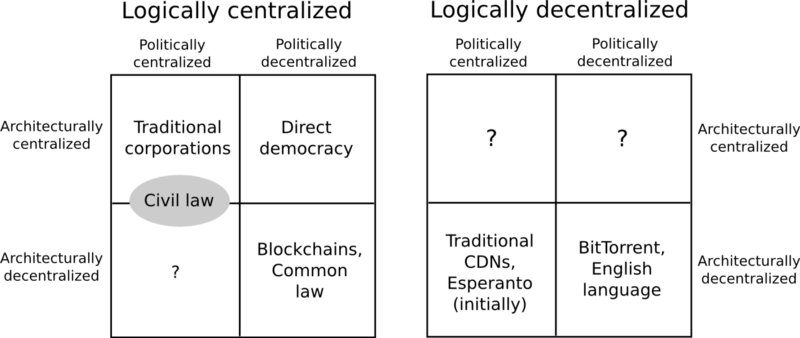
\includegraphics[width=0.75\textwidth]{3-tier-decentralization}
		\label{fig:3-tier-decentralization}
	\end{figure}
	
	Il concetto di decentralizzazione si può dividere in tre dimensioni diverse che, nonostante siano indipendenti l'una dall'altra, hanno dei punti di contatto(come visibili in figura \ref{fig:3-tier-decentralization}). 
	\begin{itemize}
		\item Architectural decentralization: indica la numerosità di quanti dispositivi è costituito il sistema e quanto è tollerata la perdita di alcuni di essi.
		\item Political decentralization: quanti individui o organizzazioni controllano i dispositivi che costituiscono collettivamente il sistema.
		\item Logical decentralization: descrive quanto sono inscindibili le interfacce e le strutture dati del sistema. Una semplice euristica è che c'è forte decentralizzazione logica se, isolate due parti del sistema esse continuano ad operare indipendentemente.
	\end{itemize}
	
	La proprietà della blockchain di presentare un'unico database consistente si riferisce alla dimensione della centralizzazione logica, ma se può essere un bene per i sistemi basati su blockchain, per sistemi come IPFS diventa una caratteristica da evitare.
	
	La centralizzazione architetturale unita alla decentralizzazione politica nei sistemi computerizzati può essere vista come la scelta da una parte di alcuni utenti di schierarsi per l'utilizzo di certi servizi piuttosto che altri. 
	
	La centralizzazione logica implica che la decentralizzazione architetturale sia più difficile da raggiungere, è stato visto con successo che le blockchain, reti di consenso decentralizzato, funzionano, ma sono più impegnative da implementare rispetto ai sistemi completamente decentralizzati architetturalmente ed indipendenti come bittorrent.
	
	Ci sono tre ragioni principali per preferire la decentralizzazione di un sistema:
	
	\begin{itemize}
		\item Fault tolerance: i sistemi decentralizzati sono meno facilmente soggetti a problemi perchè fanno affidamento su componenti separati che non dipendono l'uno dall'altro.
		\item Attack resistance : è più dispendioso attaccare un sistema decentralizzato perchè non possiede un nodo centrale facilmente attaccabile ad un costo minore.
		\item Collusion resistance: è molto più difficile per i partecipanti in un sistema decentralizzato beneficiare in qualche modo se stesso a discapito degli altri partecipanti.
	\end{itemize}
	

	\subsection{La nascita della blockchain: Bitcoin}

	Il 3 gennaio 2009, un programmatore anonimo, sotto il nome di Satoshi Nakamoto, mina con successo il primo blocco della blockchain Bitcoin dando il via alla criptovaluta più celebre di tutte e a quel processo di innovazione che oggi sta creando sempre più possibilità. Il suo articolo intitolato \textit{Bitcoin: A peer-to-peer electronic cash system}, è uno studio sulla possibilità di creare una moneta virtuale completamente autonoma e distribuita basata sulla crittografia, la proof-of-work e una rete peer-to-peer che la sostiene\cite{nakamoto2008bitcoin}. 
	Questo lavoro, pubblicato il 31 ottobre 2008, è il condensato di tanti concetti, alcuni dei quali semplici ipotesi altri veri e propri trattati teorici o progetti che nel passato erano stati diffusi. Il paper di Nakamoto è il primo documento formale contenente i concetti fondamentali che hanno preceduto la messa in funzione, poco tempo dopo, di Bitcoin, un sistema di scambio di denaro elettronico tramite una rete peer-to-peer. Nakamoto introduce la sua innovazione partendo da un problema noto che affligge il commercio in internet: l'obbligo di una terza parte fidata, come una banca, la quale con costi impraticabili non permette lo scambio di piccole somme di denaro tra due utenti. Riconosce l'assenza di un sistema di pagamento che non coinvolga terze parti e che non sconfini nell'acquisire informazioni che invadano la privacy.
	La sua soluzione è costruire un sistema basato non più sulla fiducia verso una third-trusted-party, bensì sulla crittografia.
	
	Prende spunto dal concetto di Bmoney\cite{bmoney} espresso da Wei Dai il quale idealizza un nuovo modo, indipendente ed anonimo (in quanto le persone si presentano mediante chiave pubblica e non più con le loro identità), di scambio di denaro decentralizzato utilizzando la crittografia asimmetrica a chiave pubblica e privata. 
	Nel sistema Bmoney ogni utente dispone di un database contenente il bilancio, indicizzato tramite chiave pubblica, degli altri utenti e tutte le forme di comunicazione tra di essi avvengono tramite messaggi broadcast. Idealizzò l'utilizzo di contratti tra più parti: un offerente, un compratore, un escrow \footnote{Escrow: un escrow è una terza parte del contratto e garante che vigila sul rispettato delle clausole delle parti.}, che sottoscrivevano un contratto con la possibilità di automatizzare delle funzioni nel caso non venisse rispettato. 
	Purtroppo un sistema decentralizzato di scambio di monete virtuali, per definizione, non può fare più affidamento ad un ente centrale per il conio di nuove monete, come invece accade nel caso delle monete a corso legale\footnote{Sottocapitolo \ref{sssec:chidecideilprezzo}}. Oltre a ciò bisogna prevedere un meccanismo per assegnare un valore alla criptovaluta. Wei pensò alla possibilità di coniare monete ripagando gli sforzi utilizzati per risolvere dei quesiti proposti da altri, sia intellettuali che pratici.
	E' proprio con Wei Dai che per la prima volta si può parlare di criptovaluta: il denaro migra da un bilancio all'altro mediante transazioni, esse contengono la chiave pubblica del beneficiario e l'ammontare del denaro ed il tutto viene firmato con la chiave privata del mittente così da permettere a chiunque di verificarne l'autenticità. Il problema che si presenta nella trattazione di Wei Dai è la consistenza e la condivisione di una risorsa comune, un database univoco che possa essere utilizzato per tener traccia dello storico delle transazioni allo scopo di evitare il consumo di risorse già trasferite, il c.d. \textit{double spending}. 
	
	\begin{figure}
		\caption{Catena delle transazioni o firme digitali}
		\centering
		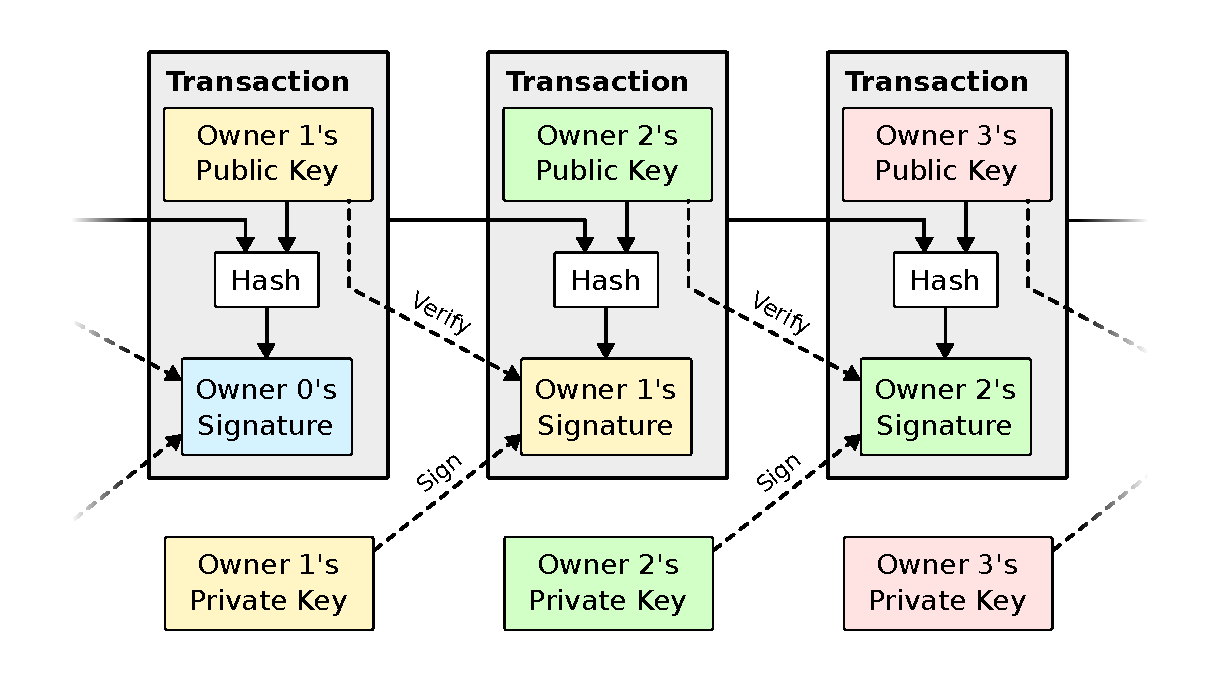
\includegraphics[width=0.75\textwidth]{transactions}
		\label{fig:transactions}
	\end{figure}
	
	Nel nuovo sistema Bitcoin vengono rielaborati i concetti di Bmoney e utilizzati per creare la catena di transazioni. Come si vede dalla figura \ref{fig:transactions} se un utente, identificato mediante una coppia di chiavi pubblica/privata, ha ricevuto a suo carico una proprietà si troverà una transazione che lo indicherà. 
	Nakamoto aggiunge delle varianti alle transazioni di Bmoney: viene applicata la funzione hash tra la chiave pubblica del destinatario e l'hash della transazione precedente (quella che ha visto l'attuale mittente essere il destinatario della moneta) e, successivamente, firmati dalla chiave privata del mittente.
	Questo porta a dare una definizione di electronic coin come una sequenza di firme digitali.
	Si pone, a questo punto della trattazione, il problema di evitare il double-spending di una singola transazione, che non può essere evitato mediante la sola concatenazione di transazioni.
	
	Una possibile soluzione è un'autorità centrale che sia a conoscenza e controlli tutte le transazioni, ma ricadiamo nel problema fondamentale della presenza di una terza parte fidata. Quindi una proposta può essere quella di rendere pubbliche le transazioni, in modo che chiunque possa controllare l'assenza di double-spending e si deve disporre di un sistema che permetta di stabilire un consenso sulle transazioni effettuate.
	Nakamoto pensò che l'utilizzo di una rete distribuita di timestamp server peer-to-peer sia la soluzione al problema del double-spending. 
	Lo scopo principale dei server di timestamp è proprio quella di raccogliere, registrare e mostrare una prova pubblica che un certo dato, dopo il momento della sua registrazione, esiste ed è precisamente quello.
	Nakamoto ancora si basa sulla letteratura passata per ideare un semplice sistema di timestamping come si può notare in figura \ref{fig:timestamp-server}.
	
		\begin{figure}
			\caption{Timestamp di elementi mediante hash}
			\centering
			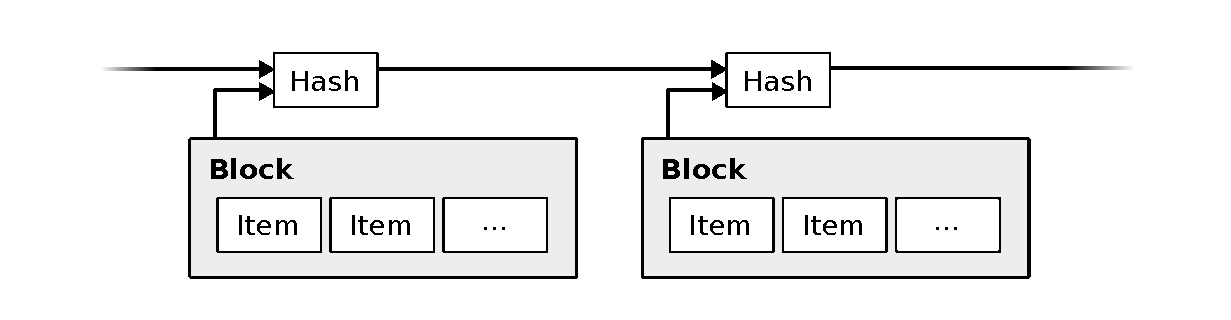
\includegraphics[width=0.75\textwidth]{timestamp-server}
			\label{fig:timestamp-server}
		\end{figure}
		
	%non so come mai ma il concetto di condivisione e ridondanza della blockchain nei nodi non si capisce
		
	Il concetto generale è quello di formare una catena,sempre crescente, composta dai valori hash ottenuti tramite l'hash dei documenti e l'hash del blocco precedente. I valori così trovati devono essere pubblicati per permettere il confronto.
	
	Ora che si dispongono gli strumenti necessari per risolvere il double-spending bisogna risolvere da una parte il problema dell'esistenza di più nodi che condividono catene diverse, dall' altra bisogna impedire che si possa facilmente modificare la catena di timestamp.
	%\%TODO guardare-> https://bytecoin.org/blog/proof-of-work/ è vero che bitcoin si basa su hashcash ma a non si può reputare ad adam l'invenzione della proof of work (il nome in realtà non è stato scritto in nessun paper) http://www.hashcash.org/papers/pvp.pdf
	Per risolvere quest'ultimo problema il sistema Bitcoin fa uso dei concetti che sono alla base di Hashcash. Originariamente Hashcash è stato un meccanismo di protezione contro l'abuso di e-mail da parte di bot o spammer \cite{back2007hashcash}. Il concetto che sta alla base di Hashchash, usato per prevenire attacchi di Spam a caselle postali, è quello di impedire che un attaccante possa trarre guadagno dall'uso indistinto di un servizio obbligandolo a consumare tempo e risorse per una determinata azione.
	
	Quello che si richiede è la dimostrazione del lavoro impiegato sia in termini di tempo che di risorse: la cosiddetta \textit{proof-of-work} \cite{liu2006proof}. 
	La proof-of-work di Hashcash è la prova della creazione di un \textit{token} mediante una CPU cost-function. Quest'ultima deve soddisfare varie proprietà, ma principalmente deve garantire che, da una parte l'esecuzione della funzione per la creazione del token deve essere un procedimento dispendioso, dall'altra la verifica della validità deve essere efficiente. 
	
	La proof of work di Bitcoin o PoW usa come CPU cost-function l'applicazione della funzione di hash SHA-256 per calcolare l'hash di un blocco in modo tale da soddisfare una determinata proprietà chiamata \textit{difficoltà}. 
	La difficoltà di un blocco indica il numero di zeri consecutivi in posizione dei bit più significativi e il lavoro medio richiesto, per soddisfare la PoW, è esponenziale nel numero di bit a zero che sono richiesti, mentre la verifica può essere fatta efficientemente mediante l’esecuzione di un numero ristretto di hash.
	Nakamoto ritiene in oltre che, in previsione dell'aumento delle prestazioni e dell'aumento dei partecipanti, la difficoltà della PoW varia in funzione del numero medio di blocchi creati in ora e, per mantenere questo valore costante, la difficoltà aumenta e diminuisce con esso.
	
	In figura \ref{fig:proof-of-work} è mostrato il contenuto di un blocco: contiene le transazioni, l'hash del blocco precedente ed un campo numerico detto \textit{nonce}. Quest'ultimo viene inizializzato a zero e, ogni volta che l'hash del blocco non soddisfa la difficoltà, viene incrementato di uno e ripetuto il calcolo della PoW finchè non viene trovato un hash valido. 
	
		\begin{figure}
			\caption{Nonce e l'hash del blocco}
			\centering
			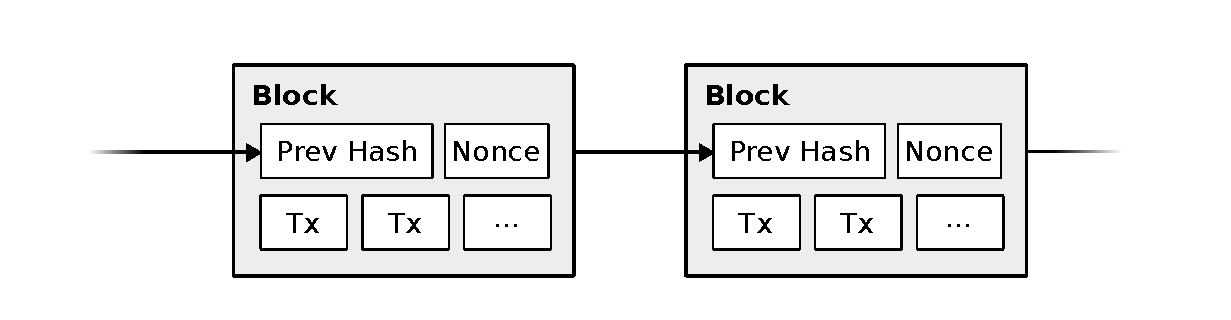
\includegraphics[width=0.75\textwidth]{proof-of-work}
			\label{fig:proof-of-work}
		\end{figure}
		
	
	Una volta che gli sforzi della CPU sono stati spesi per trovare un hash che soddisfi la proof-of-work, il blocco non può più essere modificato senza rieseguire il lavoro. Inoltre, dato che i blocchi sono concatenati l'uno all'altro, mediante l'hash del blocco precedente, modificare un blocco passato implica calcolare non solo nuovamente l'hash di quel preciso blocco, ma bensì tutte le PoW successive ad esso.
	
	Anche il consenso dei nodi su quale sia, tra le possibili catene quella \textit{migliore}, viene risolto mediante la PoW. Verrà infatti estesa solo la catena migliore, solo quella con il numero più elevato di blocchi validi.
	
	La catena più lunga gode di un lavoro e una spesa maggiore impiegata e, quindi, il modificare un blocco passato è più dispendioso da attuare rispetto alle altre. 
	Fintanto che i nodi onesti e la loro potenza computazionale rappresenteranno la maggioranza, non sarà possibile per un attaccante la modifica di un blocco passato. 
	Nakamoto definisce il comportamento di un nodo che viene informato di due nuovi blocchi validi, ma differenti.
	Prima della soluzione viene introdotto il concetto di altezza del blocco e branching. 
	L'altezza di un blocco coincide con la profondità di un nodo in una topologia ad albero dove la radice è il primo nodo minato. 
	Come si vede in figura \ref{fig:fork-blockchain}, il branching o biforcazione avviene quando un nodo riceve due blocchi validi della stessa altezza. 
	
		\begin{figure}
			\caption{Blockchain soggetta ad fork, si notano colori diversi per differenti branch.}
			\centering
			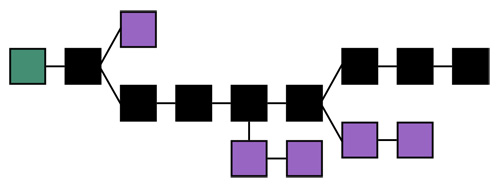
\includegraphics[width=0.75\textwidth]{fork-blockchain}
			\label{fig:fork-blockchain}
		\end{figure}
	
	
	La soluzione del problema precedente è un branching della catena: un nodo nel momento in cui riceverà due nuovi blocchi validi per la catena su cui stava lavorando, mantiene i due blocchi e costruisce una biforcazione della catena. Il nodo a seguito della biforcazione o \textit{soft fork} ha due possibili catene, entrambe valide, su cui poter lavorare per estenderle. Si tornerà a lavorare su di una sola catena nel momento in cui la lunghezza di un branch supererà quella degli altri.
	%merkle root
	Una transazione per poter essere registrata deve prima essere creata, come abbiamo visto precedentemente, e diffusa verso tutti i nodi della rete. Ogni nodo collezionerà le transazioni inserendole in un blocco e lavorerà per trovare la proof-of-work. Una volta trovata, il blocco valido sarà condiviso con tutti gli altri nodi che potranno verificare la validità e l'assenza di double-spending.
	
	La funzionalità che introdurremo nasce sempre nell'ambiente del timestamp di documenti e avrà l'obiettivo di assegnare un nome ad un documento digitale che, anche a scapito della perdita di un potere espressivo nel linguaggio umano, conferisce la capacità di identificare univocamente il documento e la sua verifica mediante crittografia\cite{massias1999design}.
	
	Come ricordiamo un timestamp è un certificato digitale che assicura l'esistenza di un certo documento in un determinato momento. 
	Attraverso la costruzione di un albero binario di valori di hash, detto \textit{Merkle Tree} dal nome del suo ideatore, si può organizzare un meccanismo rapido di verifica del timestamp dei documenti.
	Come si evince dalla figura \ref{fig:merkle-tree} l'albero viene costruito a partire dalle foglie che contengono gli hash dei documenti, ogni altro valore assegnato ad un nodo interno viene calcolato mediante l'hash dei due valori sinistro e destro a profondità successiva. Il procedimento termina fino a che non si ottiene la radice detta \textit{Round Root Value}, la quale viene combinata con il valore dell'albero precedentemente trovato calcolando l'hash e ottenendo una nuova radice detta \textit{Round Value}. 
			\begin{figure}
				\caption{Costruzione del Merkle Tree}
				\centering
				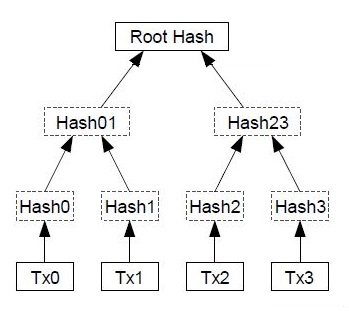
\includegraphics[width=0.45\textwidth]{merkle-tree}
				\label{fig:merkle-tree}
			\end{figure}
	Ci sono due tecniche di creazione di un sistema di timestamping : trusted-third-party e distributed-trust\cite{massias1999design}.
	Il primo per espletare la funzione di timestamp sfrutta un autorità centrale, pone i Round Value su di un sito fidato o su di un documento in modo tale da rendere i valori immutabili. Il secondo metodo invece distribuisce replica la serie di timestamp su di un gran numero di persone, basandosi sulla convinzione che corrompere un gran numero di utenti firmatari sia difficile. In ogni caso il timestamp di un documento sarà formato da tutti i valori necessari che permettono di ricostruire il merkle tree\footnote{Merkle tree o albero di Merkle dal nome del suo ideatore, e identifica un albero in cui ogni nodo interno è identificato da un hash.} a partire dall'hash del documento per poi confrontare il valore del Round Value trovato con il corrispettivo valore posto sul sistema trusted. 
	In Bitcoin l'uso è duplice, permette sia la verifica immediata dell'esistenza di una transazione senza che colui che vuole effettuare la verifica debba avere tutte le transazioni, sia permette di inserire nei blocchi, piuttosto che le intere transazioni, solo il Root Round Value o Merkle Root permettendo di alleggerirne il peso.
	
	%incentivi
	Nakamoto prevede che tutti i partecipanti della rete che riescono a soddisfare la PoW estendendo la catena, debbano percepire degli incentivi per gli sforzi compiuti. Gli incentivi, in cripto-monete, sono formati dalle tasse applicate alle transazioni e dai \textit{bounty reward} che sono il compenso per chi riesce a creare un nuovo blocco valido. 
	

	Come abbiamo già detto il problema principale di non disporre di un ente centrale, come la zecca dello stato, è che bisogna prevedere un meccanismo di introduzione di monete: per ogni nuovo blocco introdotto verranno coniate nuove monete virtuali.
	In Bitcoin è stato previsto anche uno strumento, detto \textit{halving}, che consiste nel dimezzare periodicamente il bounty reward di un blocco. Ciò consente di limitare il numero massimo di monete coniabili e quindi di combattere l'inflazione\ref{sssec:chidecideilprezzo}.
	Per far ciò la prima transazione di ogni blocco, detta \textit{coinbase} è riservata al nodo che trova la Pow e gli garantisce l'attribuzione degli incentivi.
	
	Grazie alla pubblicazione del white paper di Bitcoin e dal rilascio del codice sorgente sotto licenza MIT, nel corso del tempo sono nate nuove criptovalute basate sulla prima dette \textit{altcoin}. Le differenze tra Bitcoin e altcoin possono essere sottili e riguardare solamente alcuni aspetti implementativi, ma possono anche differire negli aspetti più profondi come gli algoritmi di consenso o funzionalità aggiuntive come anonimizzare delle transazioni.
	
	%Put simply, sidechaining is any mechanism that allows tokens from one blockchain to be securely used within a completely separate blockchain but still moved back to the original chain if necessary. By convention the original chain is normally referred to as the "main chain", while any additional blockchains which allow users to transact within them in the tokens of the main chain are referred to as "sidechains". For example, a private Ethereum-based network that had a linkage allowing ether to be securely moved from the public Ethereum main chain onto it and back would be considered to be a sidechain of the public network.
	
	Oltre a catene indipendenti, come Tenebrix, Zetacoin, Lightcoin, Dogecoin e molte altre, possiamo trovare applicazioni decentralizzate come Zerocoin o Factom che sfruttano una blockchain costruendoci al di sopra delle applicazioni indipendenti, con funzionalità aggiuntive, che possono essere a loro volta delle nuove blockchain.
	In particolare ci si riferisce a quest'ultime con il termine di \textit{sidechain} che indica ogni meccanismo che permette a delle criptomonete di una blockchain di essere usate in una catena separata, ma se necessario, possono essere riutilizzate nella catena originaria. Come nel caso di Factom nel quale si predispongono due sidechain, Factom ed Entry Credit, che permettono di operare ed aggiungere funzionaltà alla catena di Bitcoin \footnote{Il sistema di consenso di Factom. \url{https://docs.google.com/document/d/1gsXbid3UC1AwaIgmUxjsBav0WDxZi73RXIYDETdmhR8/edit}}.
	%Alcune mirano a risolvere problemi specifici come lightcoin e zerocoin
	%A tutti i livelli di utenze: dalle classiche blockchain per lo scambio di valute tra qualsiasi utenza a blockchain riservate per trasferire criptovalute tra banche come il progetto Ripple.
	
	Ogni blockchain è stata progettata per aver un preciso scopo che però limita il campo di utilizzo della blockchain da parte di nuove applicazioni, le quali sono obbligate a distribuire l'applicazione su di un sistema che usa la blockchain solo come audit.
	Questo fino alla nascita di Ethereum. 
	Ethereum si è presentata come una piattaforma decentralizzata basata su blockchain, pubblica, opensource per la pubblicazione di smart contract programmati tramite un linguaggio turing-completo. Se prima un programmatore che voleva sviluppare un'applicazione di aste online era obbligato a utilizzare due sistemi distinti, il livello applicativo basato su sistema centralizzato e la blockchain come storage, ora la blockchain non diventa solo un sistema distribuito di timestamping per criptovalute, bensì una macchina virtule capace di eseguire programmi con tutti i pro e i contro della blockchain\cite{wood2014ethereum}.
	%% potrei introdurre solo il concetto di  multitier \footnote{In software engineering, multitier architecture (often referred to as n-tier architecture) or multilayered architecture is a client–server architecture in which presentation, application processing, and data management functions are physically separated}
	

	\subsection{Proof-of-work e i problemi legata ad essa}

	Come è stato detto precedentemente l'obiettivo degli algoritmi di consenso, di cui la proof-of-work è uno di essi, è di stabilire un meccanismo attraverso il quale, in una rete blockchain pubblica, gli utenti possono riconoscere e condividere collettivamente la stessa catena. Questo permette di minimizzare la fiducia che i nodi della rete devono mantenere tra loro, permettendo l'entrata e uscita di qualsiasi nodo dalla rete in qualsiasi momento.
	Le famiglie di algoritmi di consenso utilizzati nelle blockchain sono varie e si basano su concetti differenti, ma che puntano tutte nell'utilizzare funzioni che sono impegnative da attuare, facili da verificare e che portano a stabilire delle regole per la determinazione della catena da estendere. La proof-of-work è solo una di esse, ma troviamo anche altri metodi come la proof-of-stake, proof-of-burn, proof-of-capacity.
	%https://bytecoin.org/blog/proof-of-stake-proof-of-work-comparison/
	%https://bytecoin.org/blog/proof-of-work/
	All'interno della famiglia di algoritmi di consenso basati sulla proof-of-work troviamo delle differenze negli algoritmi di cifratura utilizzati e il fattore che gli accomuna è che devono soddisfare la difficoltà, trovando un numero $x$ tale per cui l' HASH($x$) ha $N$ bit a zero.
	In pratica, l'algoritmo di hashing sarà ciò che contraddistinguerà un algoritmo di consenso da un altro. Nella trattazione orginale di Bitcoin viene utilizzato l'algoritmo di Hashcash che a sua volta si basa su SHA256. Il problema che Satoshi non si era posto inizialmente, che nel corso del tempo è stato sempre più nitido, è la differenza tra il contributo di un utente che dispone di hardware di fascia media rispetto ad un investitore che centralizza grande potenza di calcolo ( potenza di hashing). La situazione è peggiorata con l'introduzione di hardware performanti quali GPU rig\footnote{I GPU rig, letteralmente impianti Graphics Processing Unit, sono quegli apparati di calcolo parallelo che sfruttano diverse schede grafiche come singole unità di elaborazione.}, FPGA\footnote{Con l'acronimo FPGA o Field Programmable Gate Array è un dispositivo che consente la programmazione dei circuiti integrati.} e ASIC\footnote{Con l'acronimo ASIC o Application Specific Integrated Circuit si indica un circuito elettronico appositamente progettato per essere efficiente nell'esecuzione di particolari compiti.} che hanno azzerato il contributo che un utente medio poteva fornire, decentralizzando completamente la potenza di calcolo verso chi ne dispone maggiormente, o come spesso accade, chi può farlo a basso prezzo. 
	Il problema generale risiede nell'utilizzo di funzioni di hashing, come SHA1 o SHA256, che sono ideate per essere performanti. Inoltre l'unico bottleneck di queste funzioni è il numero di operazioni al secondo che un hardware può eseguire e, che rispetto alle CPU di fascia alta, può essere aumentato di vari ordini di grandezza mediante l'utilizzo di hardware dedicati (ASIC) al posto dei comuni processori. 
	Questo unito al fatto che la produzioni di ASIC e il mining è in mano a poche industrie dell'est asiatico ha posto grandi interrogativi sulla qualità della PoW di Bitcoin e su quanto sia effettivamente decentralizzato.
	
	Queste ragioni hanno spinto la blockchain \textit{Tenebrix}, nel settembre 2011, a proporre una variante della funzione crittografica SHA256 e una nuova proof-of-work che non utilizza il numero di operazioni al secondo come bottleneck, bensì operazioni che includono grandi moli di dati e maggior memoria\footnote{\url{https://bitcointalk.org/index.php?topic=45667.0}}.
	Il progetto Tenebrix puntava a ridare la possibilità a chiunque di minare questa criptovaluta traendone profitto, essendo progettato per essere inefficiente se eseguito su apparati che vengono usati per il calcolo parallelo o ASIC. Inoltre l'utilizzo di una nuova tecnologia poneva nuovi sbarramenti a chi volesse attaccare la rete mediante il superamento del 51\% di potenza di hashing, perchè non solo un attaccante avrebbe dovuto superare il 51\% di hashrate dell'intera rete, ma avrebbe dovuto investire denaro nella ricerca e sviluppo di nuovo hardware ASIC per la proof-of-work Tenebrix diminuendo la profittabilità dell'attacco.
	\textit{Scrypt}, l'algoritmo alla base della PoW della nuova blockchain, non è una funzione crittografica di hashing come lo è SHA256, ma fa parte della famiglia di funzioni di derivazione della chiave \textit{KDF} (Key Derivation Function)\cite{percival2009stronger}. In particolare queste funzioni vengono utilizzate per la memorizzazione di password nei database o, come nel caso dell'algoritmo HMAC, per l'invio di messaggi firmati che consente la verifica dell'integrità e dell'autenticità del messaggio.
	
	Le funzioni KDF nascono per aggiungere maggior sicurezza rispetto alle funzioni di hashing nel salvataggio di password nei database. In generale data $H$, una funzione KDF, dato $S$, un numero detto salt, si calcola la \textit{derivative key} $h$ di un messaggio $m$ applicando $H(m,s)$. Nelle normali funzioni hash abbiamo un solo parametro (il messaggio) che è ciò che vogliamo trovare se siamo degli attaccanti e vista la non invertibilità della funzione e la distribuzione costante delle preimmagini questo ci porta ad effettuare un attacco brute-force sull'hash del messaggio per risalire al contenuto originario. In particolare, a questo scopo, un attaccante si può appoggiare alle \textit{Rainbow Table} che contengono i valori precalcolati del messaggio e il proprio hash così da fornire l'inversa dell'hash in tempo costante. Per prevenire questo tipo di attacco le funzioni di derivazione della chiave aggiungono una difficoltà, l'hash del messaggio è parametrizzato mediante l'aggiunta di un numero random detto \textit{salt}: se un attaccante vuole conoscere l'inversa in tempo costante deve trovare l'intera rainbow table di un preciso valore salt.
	
	Le funzioni di derivazione della chiave hanno come obiettivo quello di complicare la generazione della chiave, non troppo per essere calcolata in tempi ragionevoli, ma abbastanza da prevenire utilizzi malevoli. Quelle che in teoria possono essere applicate sono le KDF adattive: in input alla funzione oltre al messaggio, il salt, viene aggiunto un parametro che aumenta il numero di iterazioni da applicare alle funzioni interne più elementari. Le funzioni KDF adattive, sono PBKDF2, bycrypt e scrypt. Questi algoritmi permettono non solo di eseguire la ricerca di un hash lentamente, o meglio, non possono essere ottimizzate mediante circuiti appositi, ma sfruttano i limiti della memoria (in termini di capacità e velocità) come limite aggiuntivo.
	
	L'utilizzo di Scrypt al posto degli altri algortimi è dettato da varie ragioni. La prima è che PBKDF2 può essere implementato efficacemente in piccoli componenti con poca RAM come gli ASIC. Bycript poteva essere un candidato ideale, ma è stato sorpassato da Scrypt sulla capacità di utilizzare intensivamente la memoria. 
	Il concetto alla base di Scrypt sono le \textit{Moderately hard, memory-bound functions} ed è stato creato da Colin Percival per ostacolare il bruteforcing nel prodotto di backup di sicurezza Tarsnap\footnote{http://www.tarsnap.com/scrypt/scrypt-slides.pdf}. 
	Si basa sull'assunzione che l'unico modo per attaccare una funzione KDF sia effettuare il bruteforcing di tutte le possibili combinazioni e la resistenza a ciò è solo questione di denaro-tempo. Come riporta Percival, il cracking di password è riducibile al calcolo parallelo, nel quale raddoppiare il numero di circuiti che processano le informazioni ne dimezza il tempo di scoperta. Quello che si può fare è incidere sul costo di produzione di questi dispositivi obbligando l'utilizzo di grandi quantità di memoria da parte dell'algoritmo di cifratura(Scrypt attualmente su litecoin alloca 128K). 
	L'algoritmo Scrypt era efficente sulle CPU che disponevano di una memoria cache abbastanza grande con la quale allocare e scambiare dati velocemente. Nel corso del tempo però vari produttori di ASIC, già conosciuti per la produzione di hardware per mining su Bitcoin, hanno creato hardware dedicato che disponga di una buona potenza di hashing su Scrypt, ma gli alti costi e le scarse prestazioni in confronto ad ASIC per il calcolo di SHA256, che erano state previste da Percival, stanno mantenendo l'hashrate delle reti delle blockchain basate su Script maggiormente distribuito.
	

	\subsection{Proof-of}
	E' stata mostrata la proof-of-work, le sue varianti in base all'algoritmo di cifratura utilizzato e la conseguenza di questa scelta, ma esistono altri metodi di determinazione del consenso.
	
	In generale una proof per essere funzionale deve rispondere a determinate caratteristiche:
		
		\begin{description}
			\item[Target]: il target è quella proprietà che deve essere soddisfatta mediante l'attuazione della proof, deve essere generato deterministicamente in modo da consentire la verifica.
			\item[Consumo di risorse]: l'attuazione del della proof comporta un consumo di risorse, sia che esse siano materiali come l'energia elettrica, sia che siano immateriali come il costo di tenere congelato un asset finanziario.
			\item[Verificabilità]: deve essere efficiente la verifica del soddisfacimento del target.
		\end{description}
	\subsubsection{Proof-of-stake}
	Il termine \textit{stake} è letteralmente tradotto in puntata, scommessa e proof-of-stake, indica la famiglia di algoritmi di consenso che si basano su quanto e come un utente possiede un'ammontare di criptovalute per garantire, allo stesso modo della proof-of-work, il consenso dei nodi della rete.
	Le criptovalute come Ethereum,Nxt e Bitshares utilizzano attualmente, o sono in procinto, di implementare nei loro sistemi la proof-of-stake, ma per comprendere al meglio i concetti che sono alla base di questo cambiamento è bene soffermarsi su Peercoin che è stata la prima blockchain ad introdurre questo nuovo concetto.%https://peercoin.net/
	Peercoin nasce nel 2012 ed è stata la prima criptovaluta a proporre un sistema alternativo di messa in sicurezza della blockchain e di incentivazione dei miner.
	
	Ciò ha permesso di introdurre nuove possibilità: se prima con la PoW veniva centralizzato il potere computazionale per rendere profittabile il mining, con l'adozione della PoS ogni dispositivo può ora competere alla creazione di nuovi blocchi per via di questo sistema leggero ed efficiente dal punto vista energetico e computazionale.
	%%peercoin white paper
	
	Peercoint sfrutta il concetto di coin age, esso non è nuovo e in Bitcoin viene utilizzato per dare la priorità alle transazioni meno recenti e non per aggiungere sicurezza alla blockchain; viene definito come segue.\\
	Data una transazione $T$  verso l'account $b$ al timestamp $t$ di un ammontare $c$, indichiamo con $T[b]_c$ l'ammontare del capitale trasferito, $T[b]_t$ il timestamp della registrazione della transazione e possiamo definire la quantità $Coinage(T[i]_c)$ nel seguente modo:
	
		\begin{equation}
		Coinage(T[b]_c) \equiv T[b]_c \times Corr(now - T[b]_t) 
		\end{equation}
	
	$Corr$ è una funzione di correzione che mappa il timestamp espresso in secondi in un'altra unità temporale e $now$ è la funzione che restituisce il timestamp attuale.
	
	Quando un'ammontare di denaro viene immesso in una transazione il coin age di quella quantità viene azzerato o \textit{consumato}.
	
	La proof-of-stake è la realizzazione dell'assunzione che per rendere sicura una rete blockchain non ci si può basare solo sulla difficoltà dell'esecuzione delle operazioni durante la fase di mining. Infatti esse spingono i miner ad investire per aumentarne la capacità di calcolo che si tramuta in transaction-fees sempre più crescenti nel momento in cui altri miner si introducono nella rete per contendersi la validazione dei blocchi.
	
	Come ogni sistema monetario la creazione di nuova valuta deve essere impedita o rallentata, se da una parte il costo della PoW è il consumo di energia-tempo, dall'altra nella PoS è il consumo di coin age e quindi la prova della proprietà di un certo ammontare che viene consumata.\\
	
	\textbf{Generazione dei blocchi}\\
	
	Nel sistema Peercoin è presente un nuovo tipo di blocco detto blocco PoS.
	
	La PoS nei nuovi tipi blocchi è una speciale transazione detta \textit{coinstake} (in riferimento anche alla \textit{coinbase} di Bitcoin) nella quale il possessore $b$ della transazione del blocco trasferisce a se stesso $T[b]_c$ consumando la quantità $Coinage(T[b]_c)$ e guadagnando il diritto di generare un blocco.
	
	In dettaglio la transazione $coinstake$ sarà formata da:
	
			\begin{equation}
			coinstake \equiv (Kernel,I)
			\end{equation}
			
	Una transazione $coinstake$ viene firmata da $b$ e sarà formata da un record di due campi:
	\begin{description}
		\item[I] : è un vettore di input non spesi, o UTXO  riferendoci sempre al sistema Bitcoin, definisce il coinage di quali transazioni passate deve essere consumato. L'indirizzo di destinazione è ovviamente lo stesso di colui che esegue la transazione.
		\item[Kernel] : è un numero che consente di modificare l'hash della transazione coinstake per soddisfare il target.
	\end{description}
	
	Nella PoW di Bitcoin è presente il campo nonce che viene incluso nel calcolo dell'hash del bocco e che permette, stabilito un target, inteso come difficoltà di mining, di ricercare l'hash che lo soddisfi. Anche nella proof-of-stake di Peercoin vengono effetuati gli hash degli input e del $Kernel$ ma il target imposto dal protocollo è dipendente dalla $coinage$ degli input. 
	
	Quando un blocco viene rilasciato, i nodi prima di accettarlo, verificano che la firma sia autentica, il valore del kernel sia corretto e che soddisfi il target imposto per colui che ha minato quel blocco.\\
	

	In questo sistema virtualmente più veloce, per via dell'assenza dell'enorme carico computazionale dato dalla difficoltà della PoW, il criterio di scelta della catena più lunga da estendere tra una serie di fork, è basato non più sulla quantità maggiore di lavoro impiegata nella costruzione della blockchain, ma sarà basato sulla quantità maggiore di $coinage$ accumulata in un ramo.
	
	In base al protocollo Peercoin durante la nascita della blockchain, quando il totale della $coinage$ è posseduta da pochi account, viene impiegata la PoW, mentre a lungo termine si utilizza la proof-of-stake.
	
	Uno dei problemi riguardanti la proof-of-stake è la facilità con la quale un nodo può lavorare su più fork della blockchain andando a competere per estenderle tutte. Peercoin e le altre blockchain basate sulla PoS risolvono questo problema in vari modi, in Peercoin viene firmato (da un'autorità trusted) un ramo che dai nodi verrà considerato il migliore.
	La soluzione proposta da Peercoin non è quella di evitare la proof-of-work, è sempre presente la possibilità di minare nuovi blocchi tramite la PoW, ma risulta più profittevole ed efficiente sfruttare ricevere gli incentivi minando tramite lo staking e quindi la PoS.
	
	\subsubsection{Proof-of-burn, proof-of-capacity e proof-of-authority }
		
	%http://www.slimcoin.club/whitepaper.pdf
	%http://www.slimcoin.club/
	
	Nel 2014 viene implementata una blockchain, \textit{Slimcoin}, la criptovaluta introduce una nuova forma di proof: la \textit{proof-of-burn}.
	Questa da una parte è simile alla PoS in quanto da la possibilità di oltrepassare l'uso della PoW, ma differisce in quanto il consumo di risorse viene inteso come consumo permanente di un certo ammontare, che ne conferisce però il diritto di minare il nuovo blocco\cite{slimecoinWhitepaper}.
	In pratica il consumo permanente viene attuato creando una transazione che non può essere riscattata da nessuno,ma che risulti facilmente verificabile.\\
	
	Nello stesso anno venne introdotta, con la moneta digitale \textit{Burstcoin}, la \textit{proof-of-capacity} che si presenta come mezzo per perseguire una più alta decentralizzazione. Il suo funzionamento si basa sulla caratteristica di essere ASIC-resistente in modo da massimizzare la profittabilità che un utente medio, con il proprio computer di casa, possa trarre dal mining, contribuendo a distribuire la potenza di calcolo. Anche se sfrutta il memory-bound è diversa dalla PoS di Litecoin perchè entrambe utilizzano quantità di memoria ben diverse e algoritmi per la determinazione del consenso diverse. Burstcoin alloca durante la sua esecuzione grandi quantità di dati, dell'ordine di diversi megabyte, denominati \textit{plot} e richiede la ricerca di particolari informazioni. Burstocoin è la prima blockchain ha presentare la capacità di eseguire codice autonomo turing-completo all'interno delle proprie transazioni.\\
	
	Infine viene considerata una proof che non richiede l'uso di risorse per minare nuovi blocchi, la \textit{proof-of-authority}, che semplicemente codifica in fase di settaggio iniziale dei nodi le chiavi pubbliche dei firmatari da cui deve essere considerata valida la creazione di un blocco e quindi trarre da essi la blockchain migliore\footnote{Proof-of-Authority: \url{https://github.com/paritytech/parity/wiki/Proof-of-Authority-Chains}}.
	
	
\iffalse	
	In tutte le definizioni troviamo delle componenti che possono comunicare tra loro sfruttando interfacce note e scambio di messaggi.
	Le caratteristiche di un sistema che lo rendono tale, si possono considerare in primo luogo l'indipendenza dei singoli computer e lo sfruttare la capacità di comunicazione e di scambio di messaggi per collaborare e cooperare. 
	Poi da questi due concetti è possibile estrapolare una serie di obiettivi che un sistema distribuito deve garantire. 
	L'accessibilità alle risorse,  deve essere intesa sia in senso proibizionista, quindi di negazione della lettura, modifica o cancellazione di dati se non si dispongono i permessi, ma anche di controllo e gestione degli accessi mediante audit. 
	L'obiettivo della \textit{trasparenza} è raggiunto mediante la creazione di un sistema che agli utenti si presenti come una singola macchina. La realizzazione di applicazioni distribuite deve basarsi su una forte astrazione, si perde il concetto di ubicazione delle risorse, la replica e la migrazione di risorse sono frequenti anche al fine di essere resistente ad attacchi e guasti di singoli nodi, i quali non devono essere percepibili dall'utilizzatore finale. Altro concetto fondamentale è la scalabilità di un sistema intesa sia come scalabilità delle dimensioni del sistema stesso, la capacità di aumentare linearmente le risorse disponibili a fronte dell'aumento di utenti, sia come scalabilità dal punto di vista geografico e da quello amministrativo. 
	La prima visione di scalabilità è una delle caratteristiche che spinge a decentralizzare qualsiasi algoritmo o servizio centralizzato: l'utilizzo di un singolo computer è il collo di bottiglia dell'intero sistema, aggiornamenti, attacchi, malfunzionamenti, costi proibitivi di aggiornamento di mainframe sono solo alcuni problemi che possono fermare l'esecuzione di un applicazione centralizzata. 
	Scalare geograficamente il sistema viene inteso sia come spezzare un componente software, e ridistribuirlo in tanti altri componenti più piccoli, sia bilanciare il carico applicativo tra i nodi. Si può dividere un algoritmo tramite approcio divid-et-impera e parallelizzare i calcoli su più nodi o possiamo semplicemente spostare il carico applicativo dal centro della rete alla periferia (i client). Quest'ultima soluzione può essere fatta non solo spostando componenti software a lato client, ma aggiungendo nuove macchine fisicamente distribuite sul territorio migliorando ritardi end-to-end. Le prime due visioni di scalabilità portano benefici su certi fronti ma introducono nuova complessità e problemi legati alla concorrenza e la consistenza delle risorse che non sempre hanno soluzioni\footnote{paxos, byzantin theorem}.
	Per la raggiunta di quest'ultimo obbiettivo possibili soluzioni possono essere la replicazione delle informazioni e la ridondanza dei calcoli unite a sistemi complessi di elezione del leader o forme di gestione Fault-Tolerance come quelle usate in diverse blockchain \footnote{Fault-tolerace Consensus http://dcg.ethz.ch/lectures/podc\_allstars/lecture/podc.pdf}.
	
	La scalabilità amministrativa, con la quale poter mantenere il controllo e la manutentibilità del sistema, spesso non è compatibile con le altre viste. La blockchain ne è l'esempio principe: i miner competono alla validazione dei blocchi e collaborano a mantenere la blockchain sicura mediante partecipazione volontaria, sono distribuiti geograficamente e sono indipendenti l'uno dall'altro. Non seguono un autorità ma, come spesso accade, sono guidati solo dal profitto che ne possono trarre. In questo ambiente d'indipendenza ma allo stesso tempo collaborazione spesso è accaduto che i miner, e le persone dietro alla loro gestione, non siano concordi con l'aggiornamento di alcune parti del codice producendo stati inconsistenti.
	
	L'approcio diffuso nell'ambiente dello sviluppo di applicazioni distribuite a partecipazione volontaria è quello di, facoltativamente, prima di condividere un'idea apertamente con gli attori del sistema, quali sviluppatori, miner e utilizzatori, e poi proporre le modifiche tramite \textit{improvement proposal} o proposta di miglioramento. Le BIP e EIP, rispettivamente \textit{Bitcoin-Improvement-Proposal} e \textit{Ethereum-Improvement-Proposal}, sono documenti per introdurre, modificare e descrivere interfacce e protocolli che sono proposti dai creatori dei sistemi distribuiti.
	
	I sistemi basati su blockchain sono architetture complesse, che constano di una componente statica, per esempio la gestione e allocazione delle transazioni così come i 'controlli' e gli algoritmi crittografici, che è creata, compilata, ma la particolarità che rende questi sistemi interessanti è la loro componente dinamica, la capacità di modificare il loro comportamento a run-time. 
	è il programma stesso che deve essere creato con la previsione di supportare questa funzionalità, la quale può essere ottenuta attraverso l'utilizzo a run-time di librerie oppure con l'implementazione di un interprete che permetta, anche da remoto, di eseguire del bytecode. Lo stesso bitcoin utilizza un interprete per un linguaggio non turing-completo basato su operazioni solo sullo stack e sui dati in input, così da permette a chiunque, in qualsiasi istante in cui la blockchain è in esecuzione, di creare, inventare ed inserire i propri metodi di pagamento personalizzati\cite{bonneau2015sok}.
	
	La blockchain risiedente su di un sistema distribuito richiede che gli aspetti di dinamicità e scalabilità vengano rispettati e le interfacce a cui i nodi si appoggiano per richiedere i servizi siano note. Supponendo che i computer siano uniformati ad utilizzare una particolare versione dell'applicazione distribuita, quindi predisporre la stessa interfaccia con cui scambiarsi messaggi, rimane un problema isolato l'aggiunta o la rimozione di un nodo che partecipa alla rete di calcolo distribuito. Una possibile soluzione può essere fatta considerando una configurazione manuale, che consiste nell'indicare quali nodi partecipano alla rete, ma pone dei grossi limiti se il numero di nodi è alto e la loro partecipazione è intermettente. Viceversa l'utilizzo dell'archittettura orientata ai servizi (Service Oriented Architecture) modellizza interfacce di registrazazione e di deregistrazione  con le quali un nodo segnala la sua partecipazione, o uscita, alla rete e può effettuare operazioni di discovery che gli consentono di scoprire quali nodi e servizi sono disponibili\footnote{http://www.d-net.research-infrastructures.eu/node/34}.
	Varie applicazioni quindi si appoggiano a servizi centralizzati o decentralizzati, come applicazioni IRC o sistemi dns, per tenere traccia di quali nodi (indirizzo ip e altri meta dati) offrono un servizio.
\fi





\subsection{Aspetti economici}

Un aspetto fondamentale introdotto da Nakamoto nella sua trattazione e in tutte le criptovalute attualmente in rete è la presenza di incentivi per i miner che consentono di guadagnare valuta digitale. In teoria questo viene attuato per consentire la decentralizzazione dei miner e della loro potenza di calcolo con lo scopo di conseguire un alto livello di sicurezza e imparzialità. Nel mercato composto da miner, utilizzatori di criptovalute, fornitori di servizi quali wallet online e side-chain considerano la criptovaluta come una vera e propria moneta al pari delle monete \textit{fiat}\footnote{Con monete fiat si intende un mezzo di pagamento legale riconosciuto dallo stato ed emesso da un'autorità, il mezzo non possiede un valore intrinseco come una riserva aurea.}.

Questa peculiarità permette ai cosiddetti \textit{exchange} di imporsi come banche decentralizzate, le quali scambiano criptovalue o valute fiat applicando un tasso di cambio. Ciò è reso possibile dal largo impiego di criptomonete nel mondo reale come mezzo di scambio tra le persone, spingendo nuovi utenti, interessati a utilizzare questi metodi di pagamento alternativi, a cercare di ottenere un certo ammontare di criptovalute accettando di scambiarlo con beni e servizi.

A sua volta questo fatto permette ai miner che spendono, anche in minima parte, tempo o denaro per rendere sicura la rete, di ricevere delle criptovalute che possono essere tramutate in denaro per ripagare i propri sforzi.

Se così non fosse le reti pubbliche basate su blockchain non potrebbero giovare più del contributo autonomo e volontario dei miner i quali non potendo più effettuare il cambio tra criptovaluta in valuta reale si troverebbero in una situazione di perdita. 

Per trarre una stima del consumo di elettricità, quindi del costo associato all'operazione di mining, possiamo moltiplicare l'hashrate (la quantità di hash al secondo della rete) per la potenza assorbita dagli apparati che effettuato l'operazione. Attualmente, la criptovaluta più diffusa della rete (Bitcoin) viene sostenuta da un hashrate di oltre $3,400,000,000 GH/s$\footnote{Stima derivata dal tempo di risoluzione della PoW, che a sua volta varia in base alla difficoltà (\url{https://blockchain.info/it/stats})}. Il costo energetico di un GigaHash, associato ai dispositivi che vengono sfruttati dai miner, è più complicato da stimare, in quanto essi impiegano una grande varietà di mezzi e tecnologie per validare i blocchi: Nonostante questo si può pensare che per via della profittabilità e dell'economicità dell'impiego di hardware ASIC e GPU, solo queste due tecnologie vengano usate. I consumi di questi dispositivi variano da 0.10 W/GH a 10 W/GH, quindi, prendendo una valore centrale come 5 W/GH, possiamo ben accorgerci di quanta potenza ed energia venga impiegata al secondo per minare la criptovaluta Bitcoin. Considerando la somma di tutte le blockchain possiamo considerarlo un valore allarmante.

L'enorme inefficienza del processo di mining (basato su PoW) porta coloro che vogliono trarne guadagno ad investire grandi capitali e spostare i propri stabilimenti dove il costo dell'energia è minore. Non a caso il maggior numero di blocchi minati viene trovato da miner e pool cinesi o dell'est europa \footnote{\url{http://www.businessinsider.com/bitcoin-pools-miners-ranked-2016-6?IR=T/\#2-antpool--1682-17}}. Se nel breve termine questo non può dare delle conseguenze, gli alti costi di gestione possono tagliare fuori qualunque altro utente indipendente dall'operazione di mining portando quei pochi miner a centralizzare sempre di più la potenza di calcolo e, di conseguenza, la decisione su quali transazioni includere o no nei blocchi.

\subsubsection{Chi decide il prezzo}\label{sssec:chidecideilprezzo}


Come ad ogni altra valuta reale, la collettività ha assegnato alle criptovalute un prezzo, inteso come costo di cambio tra una valuta e l'altra. La confusione però è molta, ma a livello europeo si è delineato cosa siano le blockchain intese in senso di valute virtuali:

\begin{description}
	\item[Valute virtuali]:  si intende una rappresentazione digitale di valore che non viene emesso da una banca centrale o da un’autorità pubblica e non necessariamente collegato a una moneta a corso legale, ma è accettato da persone fisiche o giuridiche come mezzo di pagamento e può essere trasferita, immagazzinata o scambiata elettronicamente.\footnote{ttps://www.ecb.europa.eu/pub/pdf/other/virtualcurrencyschemesen.pdf}
\end{description}

La logica che sta dietro all'assegnazione del valore di un singolo "coin", sia che la criptovaluta sia riconosciuta o meno come moneta a corso legale, è la stessa delle valute fiat. Essa si riduce, ad esempio, al chiedersi quanto vale un RMB in Euro: tutte le valute hanno un proprio valore di cambio rispetto a tutte le altre. 

Il mercato costituito dagli scambi delle valute è il Forex\footnote{Foreign exchange market o mercato valutario} e Bitcoin e le altre valute virtuali non sono incluse in esso.

Nonostante le criptovalute siano riconosciute solo come mezzo di pagamento e non come bene, esistono gli scambia valute o \textit{exchange}, i quali sono il punto di contatto tra l'ecosistema delle valute virtuali e delle monete a corso legale. 

Poloniex, Kraken, BTC-e sono solo alcuni exchange che offrono questi servizi di compravendita di criptovalute. I servizi offerti da questi enti sono vari, dalla compra-vendita e trading di qualsiasi valuta, al fornire wallet con cui gestire i propri bilanci online.\\

E' dal fenomeno di trading che si stabilisce il prezzo, in particolare si fa riferimento al modello \textit{Price taker e maker}. Esso definisce le operazioni che due entità, maker e taker, eseguono al di sopra di una piattaforma di trading interna all'exchange, entrambe operano in duplice modo:

\begin{description}
	\item[Maker]: notifica al \textit{libro degli ordini} che è intenzionato a comprare una quantità V di un bene per un determinato prezzo P, oppure a vendere un totale V per un compenso di P.
	\item[Taker]: osservando gli ordini, segnalerà la volontà di comprare V al prezzo di P (dove P è maggiore o uguale del minimo prezzo dei Maker per vendere V) o di vendere V al prezzo di P (dove é minore o uguale del massimo prezzo dei maker per comprare V).
\end{description} 

L'incontro tra una richiesta dei maker e la corrispettiva richiesta del taker che la soddisfa produrrà lo scambio tra le due entità. L'exchange potrà applicare delle tasse alle richieste dei maker e taker per incentivare o disincentivare certe operazioni o volumi scambiati\footnote{\url{https://www.kraken.com/help/fees}}.
 
L'incontro tra le offerte tra maker e taker determinerà il valore delle criptovalute, e quindi sarà molto volatile e potrà cambiare molte volte nel giro di pochi minuti. Il valore di un coin non sarà univoco, ma andrà contestualizzato a seconda di quale exchange si sta usando, in quale valuta vuole essere convertito e in che preciso istante lo si sta osservando \cite{seforo2014currency}.

\subsubsection{Halving}

In alcune reti blockchain è presente il concetto di halving che consiste nel periodico dimezzamento del bounty reward. Quest'ultimo è il compenso, in termini di criptovaluta, che il miner riceve per aver aggiunto un blocco alla catena. Nei sistemi che implementano questa funzionalità, l'halving avviene in periodi fissati (es. ogni $n$ blocchi) che portano, nel corso del tempo, ad una situazione nella quale il numero di monete prodotte per blocco sarà zero e il numero di monete prodotte avrà raggiunto il tetto massimo. Se l'implementazione potrebbe sembrare una feauture con scopi prettamente tecnici, in realtà è inserita in molte blockchain per gestire unicamente aspetti economici. Lo scopo di questa procedura è diminuire l'inflazione che l'immissione di nuova valuta può dare a lungo termine. L'inflazione determina la diminuzione del potere d'acquisto della criptovaluta, osservabile tramite il cambio rispetto a monete fiat, causato dall'introduzione nella rete blockchain di nuove monete. In Bitcoin il fatto che oltre il 75\%,rispetto al tetto massimo di 21 milioni, delle monete sia già stato introdotto in circolazione e l'halving ne riduca sempre di più l'introduzione porta ad una continua crescita del prezzo legato ad una domanda sempre più crescente per accaparrarsi il maggior numero di valuta prima che l'emissione si fermi.\\

%http://smartmoney.startupitalia.eu/bitcoin-blockchain/51665-20160202-halving-bitcoin
Un'altro aspetto importante è che i miner basano la sostenibilità dei loro sforzi dagli incentivi che la blockchain li assegna: oltre a il reward del blocco e le fee applicate alle transazioni non ci sono altri metodi interni alla blockchain per ricavare un compenso\footnote{\url{http://smartmoney.startupitalia.eu/bitcoin-blockchain/51665-20160202-halving-bitcoin}}\footnote{In altri sistemi, come Ethereum, è presente anche il concetto di Uncle che sarà analizzato nei capitoli seguenti}.

Se il reward del blocco si dimezza e i valori del cambio o delle tasse rimangono invariati molti miner non riusciranno più a sostenere i costi e si sposteranno a minare, se possibile, altre monete più proficue. Se, come in Bitcoin, le transazioni richieste superano quelle incluse nei blocchi, solo le tx con fee più alte verranno incluse portando l'aumento del valore delle fee complessivo.

Alcune blockchain non implementano l'halving perchè, come Ethereum, pensano che la somma totale delle criptovalute perse dagli utenti (attraverso la perdita delle loro chiavi o della propria password, l'invio di valuta in transazioni inspendibili) svolgerebbe in parte la stessa funzione dell'halving.


	\clearpage
	\section{Ethereum}

\iffalse
	%	https://daowiki.atlassian.net/wiki/display/DAO/Ethereum+System#
	%da tenere a mente : http://www.ethdocs.org/en/latest/
	%Spiega tutti i client che ci sono.
	%Caratteristiche del linguaggio di programmazione delle Dapp : https://forum.ethereum.org/discussion/1460/solidity-faq
	%Controllare file su drive, contiene alcune info sull'ambiente di sviluppo meteor (anche lui è un nuovo paradigma a se con client server, variabile di sessione, variabile reattive, asyncr ma )
	
	
		si discute di the DAO http://www.europarl.europa.eu/sides/getDoc.do?pubRef=-//EP//NONSGML+TA+P8-TA-2016-0228+0+DOC+PDF+V0//IT
		3 DAO tuttora, the DAO è la più famose : http://www.rischiocalcolato.it/2016/06/moneta-digitale-etehereum-colpito-dal-fallimento-the-dao.html
		\item \uncheckedbox the fact of the matter is that blockchain technology is larded through with trust. First, you need to trust the protocol of the cryptocurrency and/or DAO. This isn’t as simple as saying ‘I trust the maths’, for some actual human (or humans) wrote the code and hopefully debugged it, and we are at least trusting them to get it right, no? Well, in the case of The DAO, no, maybe they didn’t get it right.
		
		Second, you have to trust the ‘stakeholders’ (including miners) not to pull the rug out from under you with a hard fork. One of the objections to the hard fork was that it would create a precedent that the code would be changeable. But this objection exposes an unmentioned universal truth: the immutability of the blockchain is entirely a matter of trusting other humans not to fork it
		
		https://aeon.co/essays/trust-the-inside-story-of-the-rise-and-fall-of-ethereum

	\fi
\subsection{Ethereum e la sua storia}
	\iffalse
	\begin{enumerate}
		\item \uncheckedbox Che cos' è http://gavwood.com/paper.pdf
		\item \uncheckedbox Che progetti sono riusciti https://etherevolution.eu/2017/02/13/guida-ethereum-parte-2/
		\item \uncheckedbox Cosa Aggiunge alla blockchain intesa come criptovaluta 
		\item \uncheckedbox Problemi su ethereum
		\item \uncheckedbox Nuova Pow, come Litecoin si cerca di minimizzare la paralelizzabilità : https://github.com/ethereum/wiki/blob/master/Dagger-Hashimoto .
		\iffalse
		https://medium.com/@VitalikButerin/parametrizing-casper-the-decentralization-finality-time-overhead-tradeoff-3f2011672735\#.mwe6tg3j4
		Medium
		Parametrizing Casper: the decentralization/finality time/overhead tradeoff
		As Casper continues to reach an increasingly stabilized form, there has been increased interest in the various parameters that are going to…
		stando ai parametri esplicati in questo post da Vitalik, a mio parere, un passaggio al PoS avrebbe come conseguenza una riduzione sostanziale dell'economicità del sistema di mining. Ciò è evidentemente dovuto all'impossibilità di massimizzare (e minimizzare) allo stesso tempo i tra parametri chiave della funzione "  - Time to finality: how many seconds after H is proposed does H get finalized?
		- Decentralization - defined here as the size of the validator pool, eg. a blockchain might have space for 1000 active validators). Note that this corresponds directly to accessibility - the minimum amount of ETH needed to become a validator, but more on this later.
		- Overhead: how many messages per second do full nodes (including validators) need to verify?"
		Inoltre vi è da aggiungere che la semplificazione che lui adduce quando dice " Note that in reality, consensus protocols need multiple rounds of messaging, so f * o ≥ d * 2 is likely, and in normal cases more than 2/3 of nodes will show up. Hence, for convenience, let’s just use:
		
		f * o ≥ d"
		Non è per niente trascurabile, in quanto arrotonda per eccesso il parametro "decentralizzazione", necessario per minare n blocchi con x numeri di messaggi verificati dai nodi. Tale arrotondamento risulta, a mio avviso, troppo semplicistico ai fini della sicurezza dell'intero meccanismo. Poichè trascura la distinzione tra validatori "benigni" e "maligni"
		Senza considerare il paragrafo "From validator count to minimum staking ETH" in cui si evince una impossibilità di effettiva decentralizzazione dovuta al parametro "min_deposit_siz"
	
		
		%https://github.com/ethereum/wiki/wiki/JavaScript-API
		\textbf{Web3 JavaScript Ðapp API} 
		Libreria web3: permette attraverso un oggetto web3 di mettersi in comunciazione con il nodo locale tramite le chiamate RCP. Infatti web3 funziona su ogni nodo ed esponde l'RCP layer.
		\textit{esempi:}https://github.com/ethereum/web3.js/tree/master/example
		\textit{usefull pattern 4 itneraction with blockchain}:https://github.com/ethereum/web3.js/tree/master/example
		\fi
		
		\end{enumerate} 
	\fi
	
	%white paper
	Ethereum è un progetto open source divenuto operativo il 30 Luglio 2015 con la versione Frontier. Bisogna retrocedere al 2013, anno in cui si incominciava ad ideare il progetto e a scrivere le prime implementazioni del codice dei nodi in Go e C++. Come di consueto l'apertura al pubblico della blockchain è stata preceduta,nel settembre 2014, dalla pre-vendita della criptovaluta Ethereum, l'Ether, permettendo così al progetto di raccogliere circa 18 milioni di dollari. Raccolti i fondi questo ha permesso di aprire fondazioni e di proseguire con lo sviluppo. Attualmente lo stato del progetto è visionabile sulla piattaforma \textit{github} all'indirizzo \url{https://github.com/ethereum} e come si può notare lo sviluppo è su più fronti: si progetta il porting del codice dei nodi in più linguaggi, si sviluppano nuovi linguaggi orientati agli smart contract come Solidity, Viper e molto altro.
	Questo progetto è il risultato di idee precedenti dove alcune, come Bitcoin, sono state le innovazioni che sono alla base di Ethereum.
	
	Prima fra tutte la creazioni di Satoshi Nakamoto il quale ha introdotto concetti nuovi e risolto grandi ostacoli che non avevano permesso la proliferazioni di determinati sistemi. La prima innovazione è stata quella di creare una moneta basata su un sistema peer-to-peer decentralizzato. La seconda introduzione che ha dato il via allo sviluppo è stato l'utilizzo in Bitcoin della proof-of-work per garantire il consenso pubblico dei nodi sul sistema di transazioni. Nessuno prima di quel momento era riuscito a superare il problema di risolvere la concorrenza di due transazioni ed evitare il double-spending, in Bitcoin si adotta il concetto di \textit{first-to-file}: la prima transazione validata diventerà parte dello stato delle transazioni a cui la seconda transazione dovrà sottostare per essere valida\cite{nakamoto2008bitcoin}. Nel capitolo successivo verra mostrato formalmente il concetto di stato e come la proof-of-work risolve il problema.
	
	L'utilizzo della blockchain per scopi che non siano la sola gestione di criptovalute ha diversi casi di successo ma presentano tutte delle difficoltà.
	Il primo fra tutti è un sistema decentralizzato di registrazione di nomi a dominio chiamato Namecoin\cite{fromknecht2014certcoin}. Esso è un implementazione di un sistema DNS e di un \textit{Registrar} che registra i nomi sulla base del criterio di precedenza. Namecoin purtroppo basa la sua sicurezza sul protocollo di Bitcoin, una gestione della registrazione ristretta e un network molto variabile che portano le persone a non utilizzare questo sistema. Questo si traduce in una rete meno sicura a causa della bassa potenza di hash.

		
	In Ethereum è stato possibile introdurre due concetti che in Bitcoin non erano stati implementati appieno: le monete colorate e la verifica di codice interno alla blockchain. Quest'ultimo è un limite alla struttura classica della blockchain, quella basata su transazioni di criptovalute: la verifica di una transazione si riferisce solo allo stato del bilancio, bytecode eventualmente interno alle transazioni richiederebbe la verifica di tutto il codice della blockchain dal blocco di genesi\cite[SPV - Simplified Payment Verification]{nakamoto2008bitcoin}. Questo ci porta a presupporre che per implementare un linguaggio di programmazione al di sopra della blockchain sono richieste strutture dati apposite. Le monete colorate invece sono criptovalute che,mediante una transazione, viene assegnata uno speciale identificativo. Questo permette di differenziarle e quindi di disporre di pagamenti configurabili in base al colore della moneta.
	
	Questi aspetti sono implementati in Bitcoin ma presentano tutti alcuni problemi insormontabili, che si concludono con il problema più grande dell'assenza di un linguaggio turing-completo per programmare le transazioni: in bitcoin le transazioni non hanno stati intermedi, possono o non possono essere inserite nella blockchain, non è possibile effettuare cicli (in modo efficiente), creare sistemi di autenticazione a più fasi o utilizzare come input delle transazioni dati che non siano lo script di verifica basato sulle curve ellittiche.
	
	L'obiettivo di Ethereum è di dare la possibilità, attraverso poche righe di codice, di fornire un contratto intelligente che abbia codificato dentro di se lo statuto del contratto e permetta di gestire asset digitali in modo autonomo. 
	Questo viene reso possibile da una blockchain che oltre a registrare dati e transazioni, condizioni base perché ci sia scambio di denaro elettronico e possibilità di memorizzazione, salva nei blocchi anche il codice degli smart contract e lo stato della loro esecuzione\cite{yellowpaperethereum}.
	
	Nel capitolo seguente si mostrerà il funzionamento di Ethereum e il suo modello.
	
	
	
	\subsection{Ethereum e il suo funzionamento}%http://yellowpaper.io/
	Nei precedenti capitoli è stato visto il funzionamento di una blockchain partendo da quella Bitcoin e sono stati mostrati i principi e le scelte fatte in base ai problemi da risolvere. 
	La storia di Ethereum è in continua evoluzione e questo si può trovare sia nella grande attività sulle repository pubbliche, sia sui blog dei principali sviluppatori. Attraverso la consultazione di questi materiali si può apprendere il funzionamento di Ethereum.
	
	Ethereum si basa sul concetto di macchina a stati basata sulle transazioni: il primo stato contiene il blocco di genesi, una serie di transazioni racchiuse in un singolo blocco porterà il sistema in un nuovo stato. 
	
	In questo capitolo verrà utilizzata la terminologia in lingua originale per conservare chiarezza con i documenti reperibili.
	
	La struttura di base su cui è definita la macchina di Ethereum segue il seguente paradigma.
	
	\subsubsection{Il paradigma della blockchain}
	
	Uno stato potrà includere alcuni dati come i bilanci degli account, i contratti stipulati e qualunque altro dato che può essere digitalizzato.
	Le transazioni rappresentano un arco valido tra due stati validi, dove una transazione $T$ si dice valida se non porta in stati $\boldsymbol{\sigma}$ inconsistenti. Uno stato $\boldsymbol{\sigma}$ è non consistente se, per esempio, è stato ridotto un bilancio senza che ci sia stata un rispettivo aumento.
	Data una tupla di transazioni $T_i$ e uno stato $\boldsymbol{\sigma}_t$ è possibile applicare la funzione di transizione di stato di Ethereum $\Upsilon$ per ottenere un nuovo stato arbitrario tra le transazioni :
	
	\begin{equation}
	\boldsymbol{\sigma}_{t+1} \equiv \Upsilon(\boldsymbol{\sigma}_t, T_i)
	\end{equation}
	
	Data la funzione di calcolo dell'applicazione di una transazione ad uno stato della blockchain ora è possibile stabilire formalmente il risultato del calcolo di un blocco.
	Prima ricordiamo che un blocco $B$ è un record formato da $(H,(T_0,T_1,...))$ dove $H$ è l'header del blocco e $T_i$ è la transazione i-esima del blocco, spesso $(T_0,T_1,...)$ verrà indicato solo con $T$.
	Inoltre consideriamo che l'utente che riuscirà a computare l'hash del blocco, in modo tale da soddisfare la proof-of-work (mining), riceverà un compenso, il bounty reward.
	
	
	Possiamo ora trovare  la funzione $\Pi$ di transizione dei livelli dei blocchi che, dato lo stato attuale$\sigma_t$, un blocco $B$ contenente $(H,(T_0,T_1,...))$ calcola il nuovo stato $\sigma_t+1$ così come segue: 
	
	\begin{eqnarray}
		\Pi(\boldsymbol{\sigma}, B) & \equiv & \Omega(B, \Upsilon(\Upsilon(\boldsymbol{\sigma}, T_0), T_1) ...) \\
		\boldsymbol{\sigma}_{t+1} & \equiv & \Pi(\boldsymbol{\sigma}_t, B) 
	\end{eqnarray}
	
	Dove $\Omega$ è la funzione che assegna al miner il reward del blocco.
	
	%Altro aspetto comune a tutte le blockchain è il fork che è ...
	
	\subsubsection{World state}
	Lo stato globale di Ethereum alla fine di una computazione di blocco viene definito come $\boldsymbol{\sigma}$ e rappresenta il mapping tra gli indirizzi, identificatori di 160 bit, e gli stati degli account serializzati. Questa struttura dati è una particolare implementazione di un albero Merkle-Patricia ottimizzato per essere efficiente \footnote{\url{https://github.com/ethereum/wiki/wiki/Patricia-Tree}} e non viene salvata nella blockchain in quanto può essere ottenuto ricalcolando tutte le transazioni dal blocco di genesi. 
	Dati l'indirizzo $a$  e $\boldsymbol{\sigma}$ lo stato globale indichiamo con $\boldsymbol{\sigma}[a]$ lo stato $a$-esimo definito dalla seguente tupla:
	
	\begin{eqnarray}
		\boldsymbol{\sigma}[a] & \equiv & (\boldsymbol{\sigma}[a]_n,\boldsymbol{\sigma}[a]_b,\boldsymbol{\sigma}[a]_s,\boldsymbol{\sigma}[a]_c)
	\end{eqnarray}
	
	Esistono due tipologie di account in Ethereum: account posseduti da utenti esterni, quindi gestibili tramite chiave privata, e account autonomi gestiti dai contratti. Essi hanno in comune 4 campi:
	$\boldsymbol{\sigma}[a]_n$ o \textbf{nonce}: nel caso di account esterni è il numero di transazioni inviate da l'account $a$, nell'altro è il numero di contratti creati da esso.
	$\boldsymbol{\sigma}[a]_b$ o \textbf{balance}: è il bilancio in \textit{Wei} dell'account $a$.
	$\boldsymbol{\sigma}[a]_s$ o \textbf{storageRoot}: è l'hash del root node dell'albero \textit{trie} che codifica la memorizzazione di contenuti per l'account $a$.
	$\boldsymbol{\sigma}[a]_c$ o \textbf{codeHash}: è l'hash del codice per la EVM associato a questo account che verrà invocato quando questo indirizzo riceverà un messaggio di chiamata. Si distinguerà un account esterno da uno orientato ai contratti perchè nel caso di account esterni il codeHash è una stringa vuota.
	
	\subsubsection{Transazioni}
	
	Una transazione $T$ è una singola istruzione firmata crittograficamente e nell'ambiente Ethereum possiamo trovare due tipologie:
	\begin{itemize}
		\item Transazioni usate per inviare messaggi.
		\item Transazioni che permettono la creazione di nuovi account.
	\end{itemize}
	
	Per prima cosa chiariamo il concetto di \textit{Gas}.
	Esso rappresenta la quantità degli sforzi da effettuare per compiere una determinata operazione. Ad ogni operazione come somma, creazione contratto, scrittura dati, suicidio del contratto, viene assegnato un certo numero di Gas. 
	Il costo delle operazioni unito al campo gasPrice determinerà le fee applicate alla transazione.
	
	Se indichiamo con $T$ una transazione possiamo definire formalmente le due tipologie:
	
	\begin{eqnarray}
	(T_n, T_p, T_g, T_t, T_v, T_\mathbf{i}, T_w, T_r, T_s) & \text{Se} \; T_t = \varnothing\\
	(T_n, T_p, T_g, T_t, T_v, T_\mathbf{d}, T_w, T_r, T_s) & \text{otherwise}
	\end{eqnarray}
	
	Come si può osservare entrambe hanno degli elementi in comune:
	\begin{description}
		\item[nonce] o $T_n$: lo scalare rappresenta l'n-esima transazione effettuata dal mittente della transazione .%uguale a %$\sigma[a]_n+1$
		\item[gasPrice] o $T_p$: uno scalare equivalente al numero di Wei che vengono pagati per unità di \textit{Gas} per tutto il costo computazionale derivato dall'esecuzione della transazione.
		\item[gasLimit] o $T_g$: è uno scalare e rappresenta il limite di \textit{Gas} che si vuole utilizzare per la transazione, non può essere modificato ed è una quantità che viene versata anticipatamente.
		\item[to] o $T_t$: è l'indirizzo ( 160 bit ) a cui verrà recapitato il messaggio. $T_t$ se possiede tutti i bit a zero ($T_t \equiv \varnothing$) indicherà una transazione di creazione di un account. 
		\item[value] o $T_v$: rappresenta il numero di Wei da trasferire all'indirizzo $T_t$ o nel caso in cui quest'ultimo sia $\varnothing$ rappresenterà il bilancio di partenza di un'account creato.
		\item[v, r, s] o $T_w$, $T_r$, $T_s$: Rappresentano 3 firme digitali e sono usate per determinare il mittente della transazione.
	\end{description}
	
	Nel caso della tipologia di transazioni legate alla creazione di un account è aggiunto il campo: 
	\begin{description}
		\item[init] o $T_i$: è array illimitato di byte che specifica il codice per EVM che verrà eseguito durante l'inizializzazione del contratto. 
	\end{description}
	L'esecuzione del codice di \textit{init} avviene solo in fase di inizializzazione e restituisce il \textit{body} che è quella parte di codice che verrà invocata ogni volta che l'indirizzo del contratto in cui è salvato il body (tramite codeHash) riceverà un messaggio.
	
	Una transazione orientata ai messaggi invece contiene una parte complementare all'\textit{init}:
	\begin{description}
		\item[data] o $T_d$: è array illimitato di byte che viene usato come input della chiamata contenuta nel messaggio (transazione).
	\end{description}
	
	Il gasLimit come abbiamo visto determina il tetto massimo che il mittente di una transazione è disposto a spendere, in particolare $gasPrice*gasLimit$ definiranno l'ammontare dei Wei che verranno spesi nell'invio di una transazione.
	Se nell'esecuzione di una transazione la quantità di gas spesa è pari o inferiore al gasLimit al mittente della transazione verrà restituita la differenza, in caso contrario la computazione si arresterà e la transazione non sarà conclusa, ma a causa della spesa computazionale sostenuta dal miner, non verrà restituito il gas speso.
	
	\subsubsection{Blocco}\label{sssec:blocco}
	Un blocco in Ethereum è la registrazione dell'esecuzione di una serie di transazioni. Esso conterrà i risultati delle computazioni o meglio l'hash delle strutture dati che permettono di tener traccia e di rendere possibile la verifica delle esecuzioni. 
	Definiamo un blocco $B$ come un record:
	
	\begin{eqnarray}
	B \equiv (B_H, B_\mathbf{T}, B_\mathbf{U})
	\end{eqnarray}

	Dove $B_H$ è l'header del blocco, $B_T$ è la lista di transazioni e $B_U$ la lista degli \textit{uncle-blocks}. Questi ultimi sono anche definiti \textit{Ommers} e sono blocchi validi che condividono con l'attuale blocco la stessa altezza. Questo permette di aggiungere una sicurezza maggiore alla blockchain perchè i blocchi passati sono stati coperti dal nuovo blocco trovato e, anche, da tutti gli Ommer-block della rete.

	L'header $B_H$ è formato da vari campi alcuni dei quali prevedono la presenza di strutture dati precalcolate come i trie dei \textit{World State}, delle \textit{transazioni} e del \textit{Transaction Recipt}.
	I campi sono i seguenti:
	
	\begin{description}
		\item[parentHash] o $H_p$: l'hash del blocco precedente.
		\item[ommersHash] o $H_o$: l'hash della lista dei blocchi Ommer.
		\item[beneficiary] o $H_c$: l'indirizzo dell'account a cui verranno assegnate le fee del blocco.
		\item[stateRoot] o $H_r$: contiene l'hash della radice del \textit{Trie State} dopo la computazione delle transazioni.
		\item[transactionsRoot] o $H_t$: contiene l'hash della radice del Trie che contiene le Transazioni.
		\item[receiptsRoot] o $H_e$: contiene l'hash della radice del \textit{Transaction Recipts Trie}.
		\item[logsBloom] o $H_b$: contiene l'hash del filtro di Bloom che contiene i log della computazione delle transazioni, esse sono contenute nel \textit{Transaction Recipts Trie}.
		\item[difficulty] o $H_d$: rappresenta la difficoltà dell'algoritmo di PoW e viene calcolata in base al timestamp e alla difficoltà del blocco precedente .
		\item[number] o $H_i$: corrisponde al numero del blocco precedente incrementato di 1, tenendo conto che il blocco di genesi ha il campo $H_i = 0$ .
		\item[gasLimit] o $H_l$: rappresenta la somma delle quantità gasLimit nelle transazioni.
		\item[gasUsed] o $H_g$: rappresenta la quantità di Gas usata nella computazione delle transazioni.
		\item[timestamp] o $H_s$: rappresenta il tempo di creazione del blocco espresso mediante l' Unix timestamp.
		\item[extraData] o $H_x$: è un array di massimo 32 byte che contiene dati aggiuntivi.
		\item[mixHash - nonce] o $H_m$ - $H_n$: sono due hash su cui si basa la proof-of-work e permettono di verificare che è stata spesa una determinata quantità di lavoro.
	\end{description}

	\begin{figure}
		\label{fig:ethereum-arc-model}
		\caption{Modello decentralizzato}
		\centering
		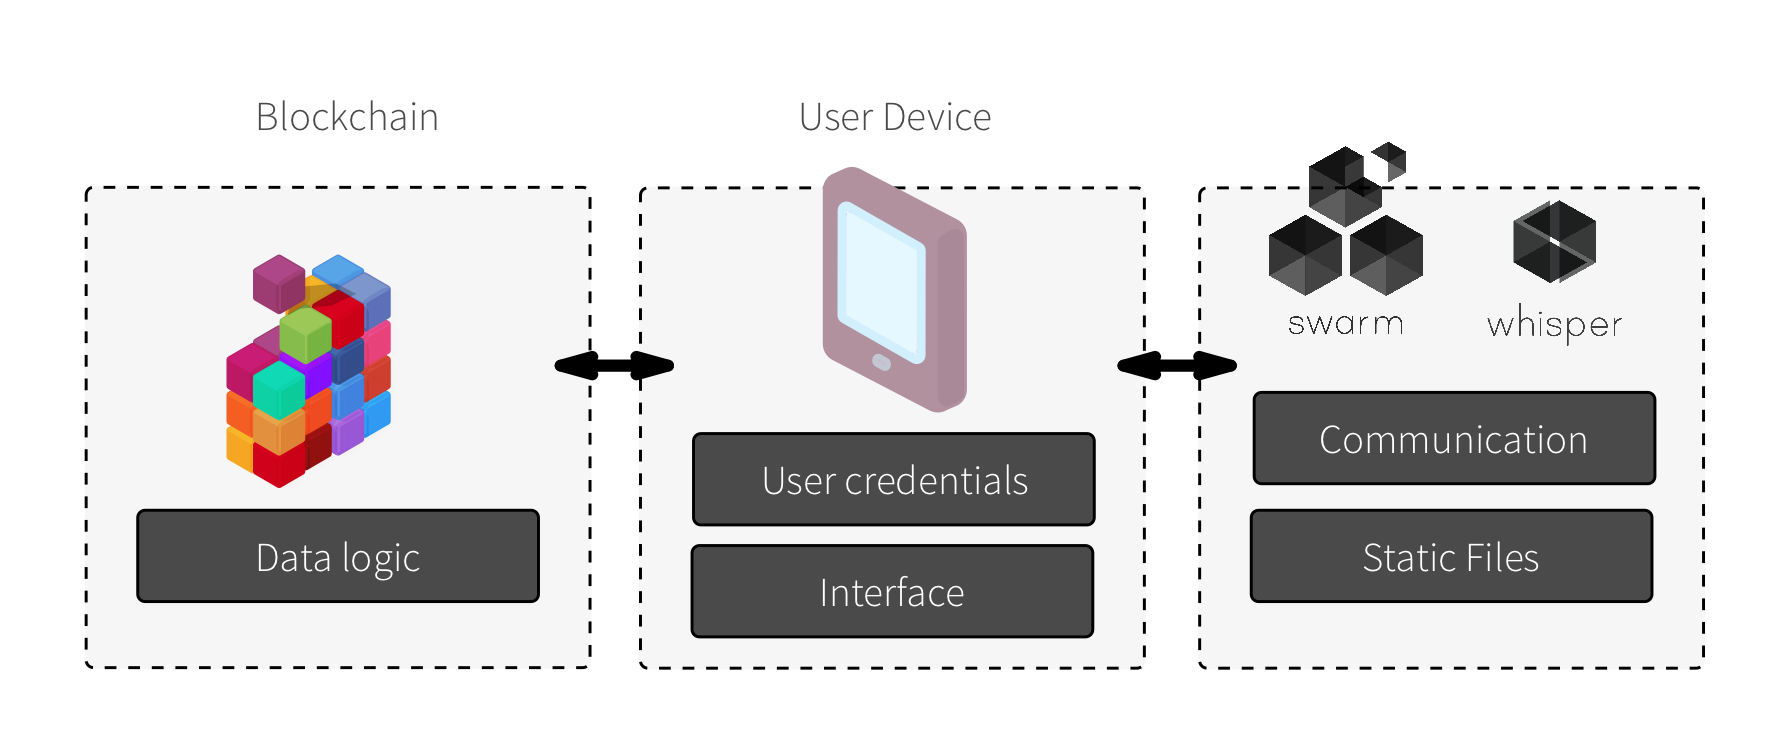
\includegraphics[width=0.75\textwidth]{ethereum-arch-model.png}
	\end{figure}
	
	\subsection{Strumenti per lo sviluppo}
	%https://blog.ethereum.org/2016/07/12/build-server-less-applications-mist/
	Ethereum vuole superare l'approccio client-server che contraddistingue gran parte delle applicazioni di rete, nelle quali troviamo un server, in cui risiedono la logica applicativa, i file statici, le credenziali dell'utente, che comunica e scambia dati con il client. Il client diviene quindi solo un interfaccia per usufruire dei servizi del server. 
	
	Un'architettura più decentralizzata, come quella di Ethereum, ci permette di disporre di un insieme di macchine e di protocolli che permettono di dividere compiti e componenti del sistema, ridistribuendone alcuni sulla macchina del client e altri in una rete peer-to-peer. Come si può osservare dalla figura \ref{fig:ethereum-arc-model}, il layer data, il quale si occupa della gestione dei dati, è affidato in mano agli smart-contract sulla blockchain, i file statici sono forniti tramite \textit{Swarm} e la comunicazione in tempo reale è gestita dal protocollo \textit{Whisper}\footnote{Whisper: è una parte del protocollo peer-to-peer di Ethereum che permette di far comunicare gli utenti attraverso lo stesso mezzo usato dalla blockchain \url{https://github.com/ethereum/wiki/wiki/Whisper}}. Il client interagirà con l'interfaccia per l'applicazione, ma dovrà gestire l'autenticazione. 
	Distribuendo l'autenticazione all'utente e affidandosi alla crittografia si solleva un server centrale della responsabilità di gestire la sicurezza di tutti i client. La distribuzione dei contenuti e la fruizione di protocolli peer-to-peer permettono di ridurre i costi e migliorare l'efficienza dei servizi.
	La divisione del layer di data con quello di presentazione permette di dare la possibilità a chiunque di personalizzare e diffondere una propria interfaccia per la stessa applicazione.

	Di seguito vengono riportati alcune componenti del sistema di Ethereum.\\
		
	\textbf{Mist}\\
	
	Mist viene presentato come l'interfaccia grafica o GUI di Ethereum o il browser per navigare nel Web 3.0 delle Dapp. In pratica è un cointaner Electron connesso a una piattaforma Meteor che permette quindi la totale programmazione degli applicativi come pagine web ( javascript,html e css ). Con esso è possibile interagire con Swarm e reperire le interfacce grafiche per le applicazioni distribuite. \\
	
	\textbf{Electrum-wallet}\\
	
	Il wallet in generale è un'applicazione che consente di connettersi ad una rete blockchain ed effettuare svariate operazioni tra cui inviare, verificare pagamenti e interagire con la blockchain tramite RPC.
	Nel caso specifico di Ethereum-wallet esso è un wallet ma è implementato come Dapp e non come applicazione stand-alone. Essendo una Dapp è stata creata per essere eseguita con meteor, è ottenibile tramite repo \footnote{\url{https://github.com/ethereum/meteor-dapp-wallet}} o via Swarm mediante Mist.\\
	
	\textbf{Swarm}\\
	
	Swarm è un piattaforma distribuita di storage oltre che un servizio di distribuzione dei contenuti, è implementato nativamente nello stack applicativo del web3 di Ethereum. Il principale obiettivo di Swarm è di provvedere una piattaforma di salvataggio distribuita e ridontante per i file relativi alle interfacce delle Dapp, che permetta l'upload di contenuti senza richiedere che il nodo debba restare connesso alla rete di peer.
	Dal punto di vista dell'utente, Swarm non è diverso dal WWW, eccetto che l'invio di informazioni non è verso uno specifico server, ma al sistema di peer. Dal punto di vista oggettivo è una piattaforma di storage peer-to-peer e fornisce soluzioni che sono resistenti a DDOS, censura, downtime e sono tolleranti ai guasti e implementano un sistema di incentivazione e di scambio della criptovaluta comune a tutte le blockchain. Swarm implementa il protocollo di rete di Ethereum devp2p e il sistema DNS di Ethereum.\\
		

\subsection{Problemi delle applicazioni basate su blockchain}\label{ssec:prolemibasatisublockchain}

La blockchain, come già riportato, è un database immutabile e non consente la modifica di un dato registrato a meno di non implementare determinati meccanismi. Questo problema trasportato in Ethereum e nel paradigma dei contratti porta all'immutabilità del codice dei contratti che sono caricati sulla blockchain. Il seguente problema verrà risolto nel sotto capitolo \ref{sssec:systemofcontracts}. Un' altra problematica di ogni applicazione di Ethereum è l'assenza della possibilità di implementare un oracolo, un generatore di numeri casuali, nella EVM di Ethereum. 
%troppo random
Il problema in prima istanza è il fallimento del consenso, della rete di nodi, sull'accettare un blocco che contiene un contratto che ha generato ed effettuato un'operazione su un valore ipoteticamente random. La funzione pseudocasuale porterà ogni nodo a determinare un valore diverso portando al rifiuto del blocco.
%poco random
Viceversa se l'oracolo è deterministico non è possibile implementare tutti quei servizi che si basano sull'estrazione casuale di un numero. 

Sulla rete si trova una soluzione \footnote{\url{https://gist.github.com/alexvandesande/259b4ffb581493ec0a1c}}a questo problema che contempla una particolare implementazione di uno smart contract e l'uso di una funzione deterministica per la generazione del numero pseudocausale. La soluzione viene trattata considerando un problema reale: la vendita di biglietti(ticket) per una lotteria a premi. Definiamo con $t[i]$ il numero del ticket comprato, con $n$ l'altezza del blocco dopo la quale l'estrazione può essere attuata e $x$ il numero di blocchi precedenti ad $n$ su cui è calcolato il numero pseudorandom(eseguento l'hash e l'operazione di modulo sui risultati ottenuti). La vendita di ticket avviene fino al blocco $t\equiv n - x - 1$ dopo il quale lo smart contract nega la vendita. Ogni utente disporrà quindi di ticket su cui non potrà inferire prima dell'estrazione finale, in quanto il calcolo sarà basato sulla creazione dei blocchi successivi a $t$. I miner potranno influenzare l'estrazione attraverso la creazione di nuovi blocchi ma non potranno decidere quale preciso ticket verrà estratto.\\

%contract alarmclock e oraclize
La EVM non ha accesso alla rete e a funzioni dipendenti dal sistema operativo che la ospita in quanto è isolata. Questo oltre a mantenere al sicuro l'esecuzione degli smart contract rappresenta, però, un problema di tutte le blockchain. Basti pensare a un contratto che vuole stimare il costo reale di un servizio, l'Ether ha un tasso di cambio e varia in funzione dell'andamento del Forex delle criptovalute. 
Oltre a questo possiamo essere interessati a richiamare la funzione di un contratto a fronte di un certo evento che può essere il superamento di una certa data temporale. 

Per questo ultimo scopo risiede nella rete principale un contratto, \textit{Ethereum Alarm-clock}\footnote{\url{http://www.ethereum-alarm-clock.com/}} che consente di schedulare eventi tra contratti e di permettere la verificabilità delle invocazioni. L'implementazione presenta alcune caratteristiche e funzionalità che consentono di prevenire l'abuso di questo contratto, ma ovviamente esso si affida all'esecuzione di processi esterni\footnote{Come recita la documentazione: `` Execution guarantees: You may have noted at this point that this service relies on external parties to initiate the execution of these transactions. This means that it is possible that your transaction will not be executed at all. In an ideal situation, there is a sufficient volume of scheduled transactions that operating a server to execute these transactions is a profitable endeavor. The reality is that I operate between 3-5 execution servers dedicated filling this role until there is sufficient volume that I am confident I can turn those servers off or until it is no longer feasible for me to continue paying their costs''.}.


Un altro sistema esterno alla blockchain che permette di disporre maggiori funzionalità, rispetto al sistema Alarm-clock, è \textit{Oraclize}\footnote{\url{http://www.oraclize.it/}}, esso si presenta come il gateway verso Internet per le blockchain per Ethereum e Bitcoin. E' un sistema molto complesso che permette di predisporre di un contratto e di API con le quali si accede alle funzionalità infinite della rete\footnote{ Utili api che possono essere utilizzate attraverso Oraclize sono per esempio quelle di Wolframaplha  \url{https://docs.oraclize.it/\#ethereum-integration-simple-query}}. In Internet l'autenticità e l'integrità dei dati via web viene garantità dall'utilizzo del protocollo https e terze parti fidate (CA come Verisign, GlobalSign, ecc.). Questa architettura si contrappone all'infrastruttura trust-less che risiede nelle blockchain ed Oraclize punta a sostituire l'autenticità dei dati, effettuata mediante terze-parti, con l'\textit{authenticity proof}.


	\subsection{Sviluppare in Solidity}\label{sssec:sviluppareinsolidity}
	% https://blog.aragon.one/library-driven-development-in-solidity-2bebcaf88736#.aleyub1u2
	%https://solidity.readthedocs.io/en/develop
	Abbiamo visto che la EVM esegue un proprio bytecode, infatti è possibile programmare in assembly-ethereum il proprio contratto. Ovviamente ciò è complicato e richiederebbe fin troppo tempo a scrivere un programma efficiente e la manutenibilità sarebbe difficile da ottenere.
	Per questo sono stati creati linguaggi di più alto livello, come Serpent, Viper e Solidity, che permettono la stesura di codice ad alto livello che una volta compilato può essere eseguito nella rete Ethereum.
	
	In generale la EVM ha delle limitazioni:
		\begin{enumerate}
			\item è isolata dal sistema operativo e un altra funzione di un altro contratto e invocabile solo se si conosce il suo indirizzo e la relativa interfaccia (ABI).
			\item Ogni istruzione della EVM ha un costo e l'esecuzione può sollevare un'eccezione in base alla quantità di \textit{GasLimit} contenuta nella transazioni, non possono essere eseguite operazioni intensive.
			\item Una volta creato il contratto non è possibile modificarlo. 
		\end{enumerate}
			
	%https://ethereumclassic.github.io/blog/2017-03-13-viper/ unsafe
	La scelta di quale linguaggio utilizzare è ricaduta su Solidity, che è un linguaggio ad alto livello orientato ai contratti staticamente tipizzato, che permette di scrivere smart contract che supportano l'ereditarietà, implementano funzioni di librerie esterne e utilizzano nuovi tipi definiti dall'utente. Solc è il compilatore per il linguaggio Solidity consente, dati una serie di contratti, di produrre il bytecode per la EVM, la documentazione, le interfacce abi. %https://www.npmjs.com/package/solc
	%descrizione di solidity
	
	Prima di discutere delle innovazioni che porta è bene far precedere dei concetti di questo linguaggio.
		
\begin{lstlisting}
contract A{
	uint amount;
	function A() payable {
		B b = new B();
		amount=msg.value - b.bbb();
	}
}

contract B{
	function bbb() returns (uint){
		return 42;
	}
}
\end{lstlisting}
		
		La principale entità che può essere creata è il contratto e, come i linguaggi OOL, esso presenta un costruttore, una funzione omonima che viene richiamata solo durante il deploy del contratto, le altre funzioni potranno essere invocate in ogni altro momento su un'istanza del contratto.
		
		Eseguendo il codice nella rete di Ethereum ovviamente avremo a disposizione una sintassi e dei costrutti specifici per gestire i pagamenti ai contratti: la label $payable$ informa al compilatore che la funzione $a()$ può accettare $b$ Ether da una transazione e l'istruzione $msg.value$ restituirà l'ammontare $b$.
		
		I contratti dispongono della possibilità di interagire tra di loro comunicando tramite le medesime modalità con le quali un account esterno interagisce con un contratto (call esterna) oppure mediante chiamate speciali che consentono di eseguire funzioni nell'ambiente del contratto chiamante (delegate-call)\footnote{Per maggiori informazioni: \url{http://solidity.readthedocs.io/en/develop/introduction-to-smart-contracts.html?highlight=delegatecall\#delegatecall-callcode-and-libraries}}.
		
		La prima modalità è una chiamata nella quale un contratto può specificare la quantità rimanente di gas nel GasLimit per la chiamata, l'ammontare di Ether da inviare e il payload. Il contratto ricevente, che può essere lo stesso chiamante, allocherà nuova memoria e potrà accedere al payload per eseguire la chiamata.
		Viceversa una delegate-call eseguirà le funzioni nell'ambiente del contratto chiamante e quindi l'ammontare del gas rimasto e per esempio le chiamate a libreria come $msg.value, msg.sig$ e tutte le altre proprietà di $msg$ riporteranno lo stesso valore.
		
		L'innovazione progettuale di Solidity si fonda proprio sull'utilizzo di librerie e sull'invocazione di delegate-call verso esse.

		I contratti come tutti gli account di Ethereum vengono referenziati tramite il loro indirizzo univoco a 160 bit e l' \textit{application binary interface} (ABI).
	
		\begin{multicols}{2}
			 Interfaccia:
			\begin{lstlisting}
[{"constant":false
,"inputs":[]
,"name":"addr"
,"outputs":[{"name":""
			  ,"type":"address"}]
,"payable":false
,"type":"function"}]
			\end{lstlisting}
			\columnbreak
			Codice:
			\begin{lstlisting}
contract A{
	function addr() returns (address){
		return msg.sender;
	}
}
			\end{lstlisting}
		\end{multicols}
		
		%https://github.com/ethereum/wiki/wiki/Ethereum-Contract-ABI
		L'ABI di un contratto è statica e viene determinata in fase di compilazione; è composta dai nomi delle chiamate a funzione, dai tipi degli argomenti e dai valori di ritorno, nonchè eventualmente da precondizioni, postcondizioni e invarianti.
		
		Dopo quest'introduzione su alcune funzionalità del linguaggio possiamo trattare le librerie e il $library driven developement$ in Solidity.
		
		Una libreria è un contratto che non può avere un bilancio in Ether, questo viene assicurato dal compilatore e tutte le chiamate a funzione verso esso sono delle delegate-call.
				 %  using CounterLib for CounterLib.Counter;
				 % self
		Il deploy di un contratto consiste nell'effettuare una transazione speciale con il bytecode del contratto inserito nel payload verso un indirizzo speciale.
		Il bytecode ottenuto dalla compilazione di un contratto, che dipende da una libreria pre-caricata nella blockchain, non può essere registrato su di essa perché l'indirizzo della libreria deve essere linkata nel bytecode del contratto. 
		
		Nel caso di un contratto che utilizza una libreria chiamata Library potremmo trovare nel bytecode un place holder simile a \_\_Untitled:Library\_\_\_\_ che indica il punto in cui inserire l'indirizzo della libreria contenuta nella blockchain.
	 
		Il paradigma della blockchain applicato al codice è di dare la possibilità di usufruire di qualsiasi libreria scritta e registrata da altri, risparmiando il costo e lo spazio sulla catena con la conseguenza di poter disporre di librerie sicure.
		
		Inoltre il paradigma dove ogni operazione ha un costo può essere utilizzato per disincentivare gli account (esterni e non) a non abusare della rete. In Solidity la funzione \lstinline|return;| trova il suo utilizzo nelle call, nelle chiamate che non hanno side-effect\ref{appendice:c}. Il comando interrompe l'esecuzione di una funzione e la EVM ritorna all'esecuzione del codice chiamante, se esistente, se no ritorna il valore alla console. La funzione \lstinline|throw;| invece solleva un eccezione: nel caso di call(dove non viene eseguita una transazione) non viene consumato del gas/ether, ma nel caso di transazioni consuma tutto il gas inserito nella transazione(normalmente se avanza del gas da una computazione viene restituito il rimanente). Il comando \lstinline|throw;| può essere catturato mediante catch, ma se viene propagato può essere usato come strumento per punire economicamente un account.
		
		Solidity è un linguaggio creato recentemente, esso è in fase di sviluppo e tante operazioni non sono possibili, per esempio non è possibile restituire un'istanza di un tipo creato da una funzione e non esistono i tipi primitivi double e float.
		A prescindere da ciò Solidity e la blockchain introducono un interessante modo di sviluppo di applicazioni distribuite. 
		

	\clearpage
	% nodo geth in ascolto sulla rete di due console 


\section{L'applicazione}\label{ssec:Progettazione}
	Lo scopo della seguente ricerca è l'implementazione di un'applicativo finalizzato alla gestione delle opere autoriali. Esso consente la registrazione, la visione di opere autoriali e la classifica delle stesse in base all'utilizzo reale degli utenti. Il sistema sarà implementato mediante smart contract in esecuzione sulla piattaforma Ethereum, ciò consentirà di disporre delle proprietà di trasparenza, tracciabilità e immutabilità proprie della blockchain.\\
	
	Verrà utilizzata la seguente terminologia:
	\begin{description}
		\item[Utente] o account: è la persona che sottoscrive la registrazione di un opera (proprietario) o acquista il diritto all'utilizzo di una determinata opera(compratore).
		\item[Opera]: è l'opera creativa, identificata tramite i metadati che il proprietario inserisce in fase di registrazione.
		\item[Contratto di registrazione] o registrazione: rappresenta la prova verificabile della cessione del diritto di utilizzo dell'opera.
		\item[Digichain] o libro mastro o ledger: è l'entità decentralizzata che gestisce l'interazione tra le componenti, è unico e da esso è possibile esercitare tutte le operazioni permesse.
	\end{description}
	
	Anche se lo sviluppo di smart contract si è concentrato sull'applicazione \textit{Digichain}, sono stati sviluppati altri contratti tra cui \textit{GlobalRegistrar} che consente di condividere in modo immediato un indirizzo tramite un nome simbolico. Questo permette di non dover più comunicare l'indirizzo di un contratto mediante sistemi esterni alla blockchain, ma più semplicemente sfruttare il concetto di database e smart contract per implementare un ente di registrazione. 
	
	\subsection{Registrar}
	
	In Ethereum ogni account, che sia uno smart contract o un utente esterno, viene identificato mediante indirizzo univoco a 160bit. Quando un utente vuole spedire un certo ammontare di Ether o vuole eseguire una chiamata ad un contratto deve recuperare in tutti e due i casi l'indirizzo del destinatario e, solo nell'ultimo, deve reperire l'abi del contratto\footnote{Riferirsi al capitolo \ref{sssec:sviluppareinsolidity}}. Per l'ultimo caso, visto che è alquanto dispendioso l'inserimento nella blockchain dell'intera interfaccia delle chiamate del contratto, nella main-chain di Ethereum l'abi viene fornito tramite Swarm. Per gli indirizzi è possibile implementare un servizio efficiente di \textit{name registrar} basato su blockchain, esso permette di:
	\begin{itemize}
		\item registrare sotto un nome simbolico un indirizzo a 160 bit.
		\item dato il nome simbolico reperire, se presente, l'eventuale indirizzo accoppiato.
		\item verificare la proprietà della registrazione di una coppia \textit{<nome\_simbolico,indirizzo>}.
	\end{itemize}
	
	
	In figura \ref{fig:globalregistrar} è possibile vedere il contratto \textit{GlobalRegistrar} che estende due contratti: \textit{Name2Address} che implementa la correlazione degli indirizzi ai nomi e \textit{Address2Name} che fornisce la funzionalità di raggruppare i nomi registrati da un utente.
	
		\begin{figure}
			\caption{Registrar}
			\centering
			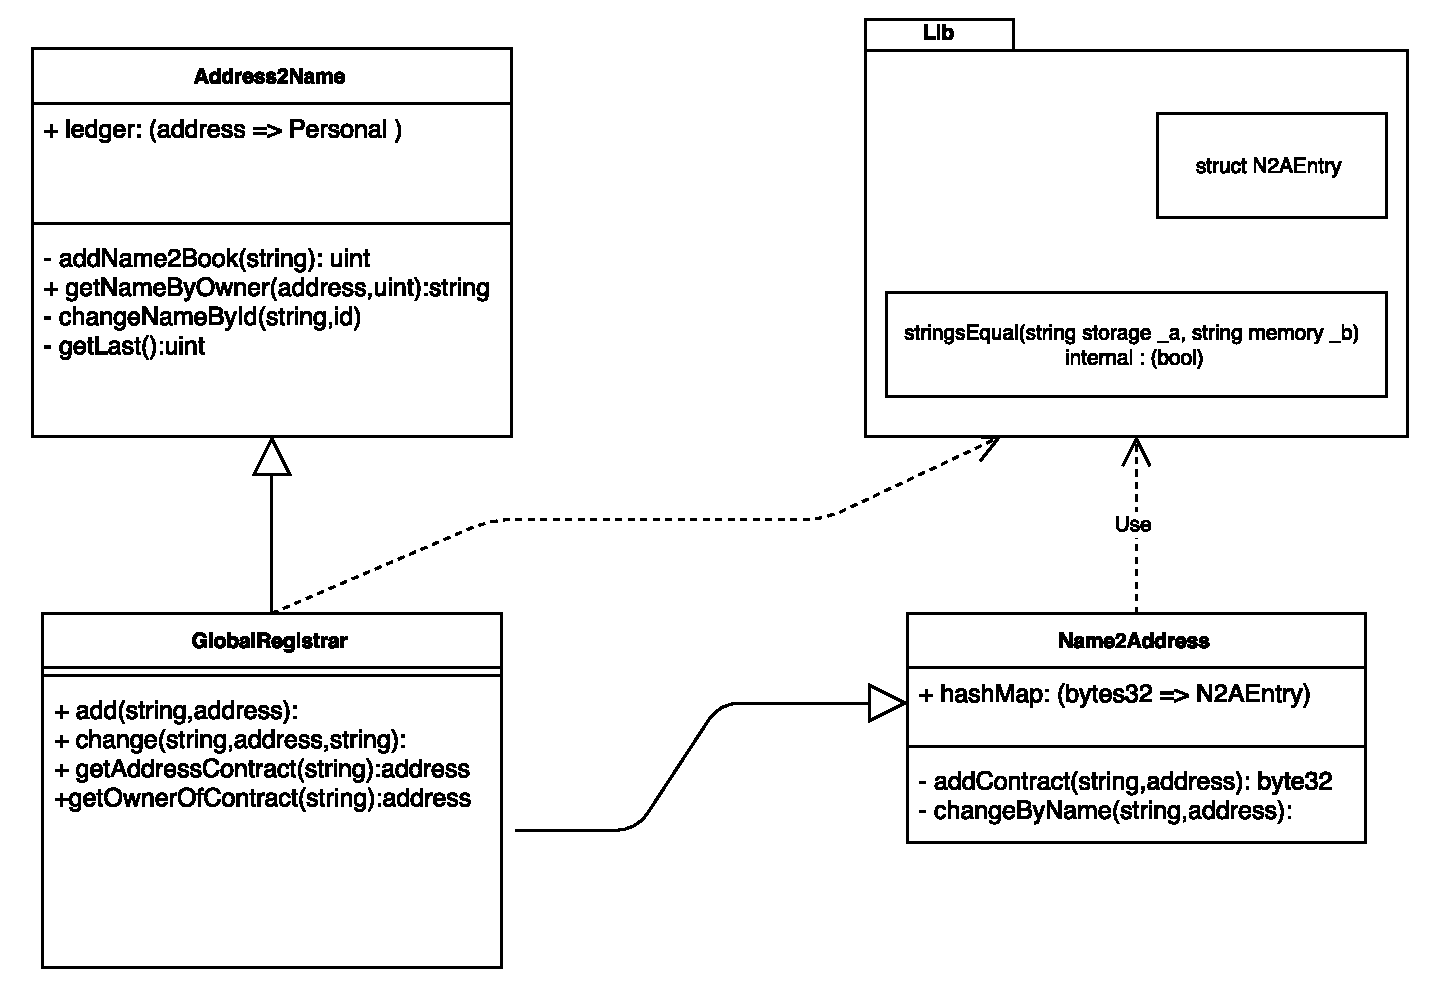
\includegraphics[width=0.75\textwidth]{GlobalRegistrar.pdf}
			\label{fig:globalregistrar}
		\end{figure}
		
	Il container \lstinline|globalRegistrar| contenuto in $GlobalRegistrar.js$ fornisce dei metodi con cui inizializzare l'istanza di un globalRegistrar, il cui codice è già caricato nella blockchain e il cui indirizzo è stato pre-caricato nel file javascript.
	
	
	
	\begin{lstlisting}
> glb = globalRegistrar.getGlobalRegistrar() 
> glb.add.sendTransaction("nomeSimbolico","0x438dfd4dfd26a42961",{from: eth.coinbase})	
	\end{lstlisting}
	
	La variabile \lstinline|glb| contiene l'istanza che collega l'abi e l'indirizzo del contratto Ethereum precedentemente caricato\footnote{Si suppone che l'utente stia lavorando connesso a una blockchain nella quale sia già stato fatto il deploy del contratto GlobalRegistrar e abbia pre-caricato l'ambiente contenente i file \lstinline|*.js|.}:
	
	Come si può vedere la registrazione della coppia di valori avviene tramite una transazione con side-effect\footnote{Consultare l'appendice \ref{appendice:b}.}.
	
	L'interrogazione del contratto, per la richiesta dell'indirizzo associato ad un nome, avviene mediante il metodo \lstinline|.getAddressContract("nomeSimbolico")|. 
	Un utente, interessato alle nuove registrazioni che vengono salvate nella blockchain, può mettersi in ascolto degli eventi lanciati dal contratto stesso \footnote{Consultare l'appendice  \ref{appendice:c} e al sotto capitolo \ref{sssec:blocco}.} che riportano dati informativi:
	
	\begin{lstlisting}
	> watcher = globalRegistrar.watchEventNewContract(glb)
	
	Nuova entry : < nomeSimbolico | 0xdfd5c578c9f5a448e71bf69cd4789211b7d94494> da l'account : 0x438dfd4dfd26a42961d878a1e27eb9f40abb0d19 .
	\end{lstlisting}

	Se due utenti vogliono registrare sotto lo stesso nome due indirizzi qualsiasi, vige il criterio \textit{first-to-file},cioè il primo arrivato acquisisce il privilegio di poter registrare e modificare l'indirizzo del nome registrato.
	Il contratto impedirà ad ogni utente di modificare record che non siano di sua proprietà e applicherà delle sanzioni nel caso venga rilevato un tentativo\footnote{Le sanzioni sfruttano i side-effect del comando throw\ref{sssec:sviluppareinsolidity}.}.

	\subsection{Digichain}
	
	Digichain è lo smart contract per la gestione delle opere autoriali. Sfruttando il contratto GlobalRegistrar gli utenti possono interagire collettivamente con il medesimo smart contract digichain semplicemente accordandosi sul suo nome simbolico.
	
	Lo smart contract consente:
	\begin{itemize}
		\item la registrazione di opere autoriali e la specifica dei metadati che la riguardano.
		\item la consultazione delle opere presenti, nonchè delle loro caratteristiche.
		\item la compravendita temporanea di opere e la verifica dello stato della cessione.
		\item la verifica della \textit{reputazione} dell'opera.
		\item la rivalsa da parte dell'autore dell'opera di rimuovere il diritto concesso al compratore in casi specifici.
	\end{itemize}
	
	Con il termine \textit{reputazione} di un opera si intende la somma di \textit{ore\_di\_utilizzo * costo\_tempo\_opera} che le persone hanno speso nell'usufruire dell'opera. Questo consentirà a tutti gli utenti di visionare la reputazione di ogni opera per scegliere quella più opportuna.
	\\

	
	Un opera è identificata tramite:
	\begin{description}
		\item[owner]: l'indirizzo del proprietario dell'opera. 
		\item[nome]: il nome dell'opera.
		\item[costoBase]: definisce in Wei l'ammontare minimo che un acquirente deve pagare per poter godere temporaneamente dell'opera.
		\item[costoTempo]: definisce in Wei il costo al minuto che un utente pagherà per usufruirne.
		\item[reputazione]: è il valore della reputazione acquisita nel corso della vita dell'opera.
	\end{description}
	
	\textbf{Registrazione}\\
	
	Un utente, allo scopo di interagire con il contratto Digichain, è obbligato a acquisire una sua istanza. Ciò si ottiene, per esempio, tramite l'istanza GlobalRegistrar nel seguente modo:
	
\begin{lstlisting}
> digichain=deployer.getIstanceFromAbiAndAddress(
	compiled.contracts["Digichain.sol:Digichain"].abi
	,glb.getAddressContract("digichain")
	)	
\end{lstlisting}
	
	Ottenuta l'istanza \lstinline|digichain|, su di essa un utente può invocare il metodo \lstinline|.creaOpera()| al quale passare i metadati dell'opera(\lstinline|(string titolo,uint256 costoBase,uint256 costoTempo)|) ed incapsulare il tutto in una transazione. 
	
	\begin{lstlisting}
	> costoBase = 200000
	> costoTempo = 10000
	> titolo = "Il titolo di questa opera"
	> digichain.creaOpera.sendTransaction(titolo, costoBase, costoTempo,{from: eth.account[0]})
	\end{lstlisting}
	
	Se la transazione è spedita correttamente\footnote{Le transazioni } ed inclusa in un blocco valido, il contratto Digichain avrà memorizzato sulla blockchain l'opera appena creata che sarà visibile a tutti tramite la call \lstinline|digichain.opere(idOpera)|.\\
	
	\textbf{Cessione del diritto}\\
	
	Ogni utente, che non sia colui che ha registrato l'opera, ha la possibilità, versando un ammontare $b$ maggiore o uguale al $costoBase$ dell'opera, di acquisire il diritto di utilizzo della stessa.

	Questo avviene attraverso i seguenti comandi:
	
\begin{lstlisting}
> bilancio = 5000000
> idOpera = 2
> digichain.compra.sendTransaction(idOpera,{from: eth.account[0],value: bilancio})
\end{lstlisting}

	Il pagamento per l'acquisto del diritto effettuato allo smart contract Digichain produrrà un nuovo contratto $R$ \textit{Registrazione} che lega l'acquirente, l'opera e l'ente di gestione delle opere Digichain. Qualsiasi operazione sul contratto $R$ appena creato potrà passare solo dalla gestione dello smart contract Digichain. 
	Se $t_0$ è il tempo di creazione del contratto $R$, indichiamo con $c$ il costo accumulato associato all'uso dell'opera nell'istante $t_1$ ed è uguale al prodotto $(t_1 - t_0) \cdot costoTempo$.
	
	Il possesso del diritto decade in due casi: se la spesa dell'utilizzo dell'opera ha superato il bilancio inizialmente versato oppure se il compratore recede dal contratto.\\
	\\
	\textbf{Recessione}\\
	
	In ogni istante, un utente che ha acquisito un diritto di utilizzo di un'opera può recedere dal contratto attraverso l'invocazione l'invio di una transazione sul metodo \lstinline|digichain.rinuncia()|. La recessione viene richiesta allo smart contract Digichain e ciò comporta la cancellazione del contratto $R$. Durante questa operazione la differenza tra il bilancio $b$ depositato in $R$ e il costo accumulato $c$ viene restituita all'utente che ha recesso, mentre, la quantità $c$ viene accreditata sul bilancio del proprietario dell'opera. Nel caso in cui il costo accumulato sia maggiore del bilancio depositato, quest'ultimo verrà interamente trasferito al creatore dell'opera.\\
	 
	%atrent forse? diagramma stati dei bilanci per rendere più chiari i movimenti nei casi in cui b>=c e b<c
	
	\textbf{Rivalsa}\\
	
	Come è stato descritto precedentemente, quando il costo accumulato supera il bilancio depositato non si scatena alcun evento\footnote{In Ethereum, come è stato osservato precedentemente, non possono essere costruiti, senza l'ausilio di sistemi (centralizzati) esterni dei meccanismi che prevedano lo scatenarsi di eventi sulla base di stati dell'esecuzione dei contratti}. Solo in questo caso specifico dove, nonostante il contratto scaduto risulti ancora registrato, il proprietario dell'opera può avvalersi del diritto di rivalsa e, e richiamando il metodo \lstinline|digichain.rinuncia()|, rimuovere personalmente il contratto sbloccando il pagamento verso di lui.\\
	

	
	Come si può vedere dalla figura \ref{fig:class-diagram} il contratto \textit{Digichain} estende la classe astratta \textit{Dao}. Questo viene fatto per dare la possibilità ad ognuno di creare la propria implementazione Digichain, anche nella previsione futura di una possibile interazione tra varie istanze Digichain specializzate in opere specifiche. L'aggregazione \textit{gestisce} mette in associazione un'istanza Digichain con $0$ o $n$ contratti Registrazione. 
	
	
			\begin{figure}
				\caption{Class diagram}
				\centering
				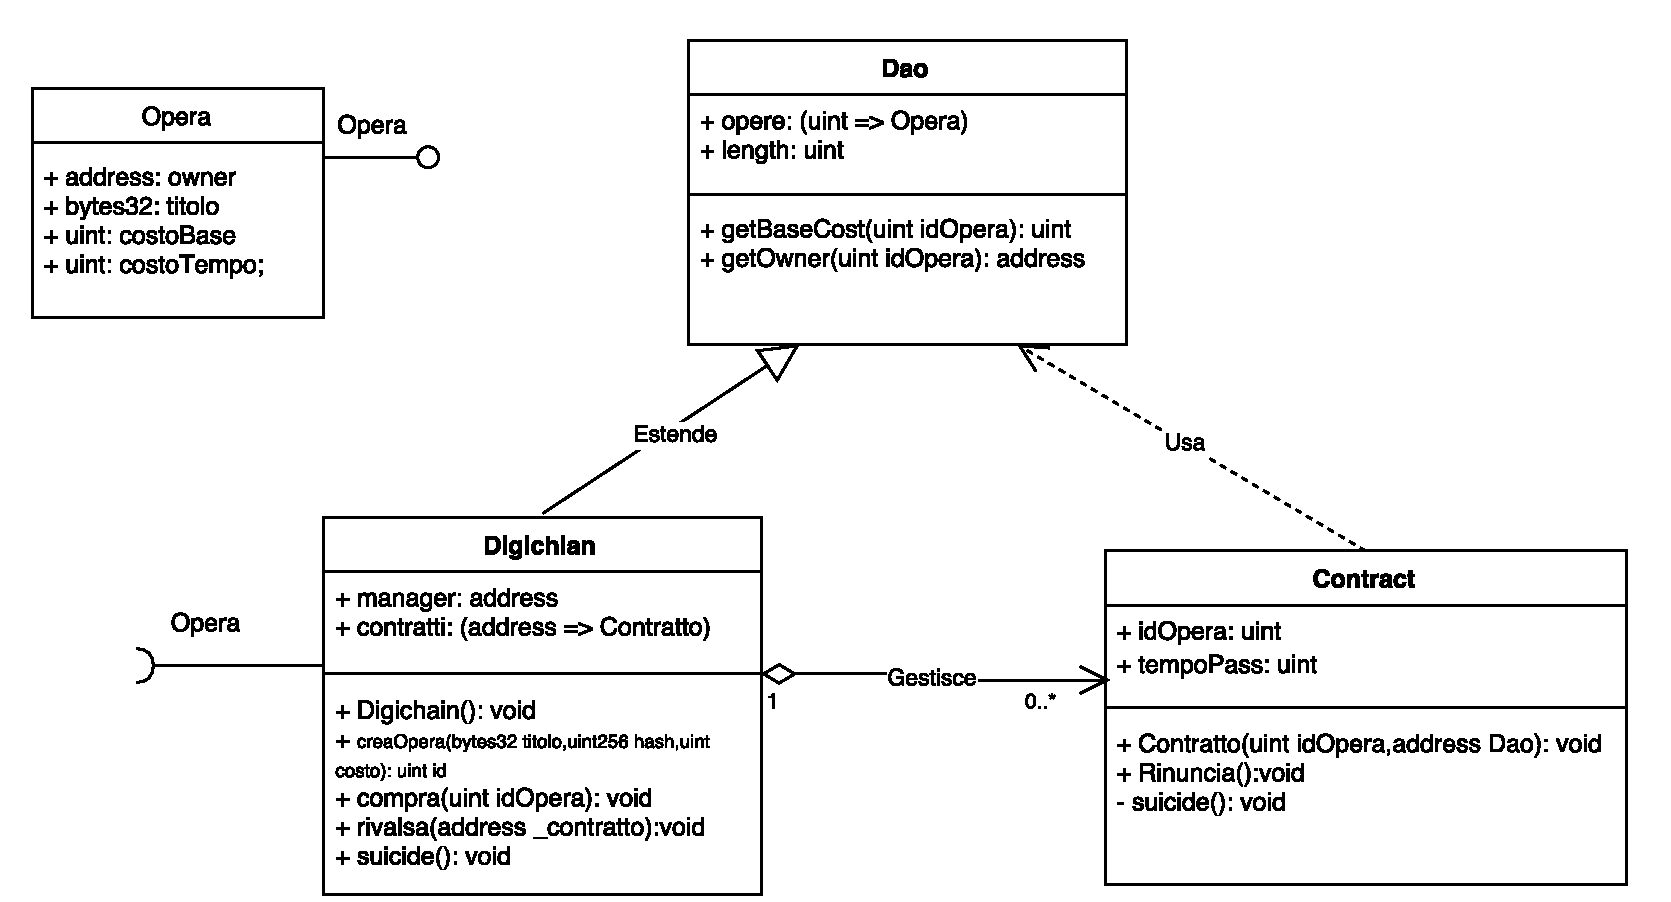
\includegraphics[width=0.75\textwidth]{class-diagram.pdf}
				\label{fig:class-diagram}
			\end{figure}
	
	
	
	\subsection{Possibili sviluppi}
	
	Ci sono diverse funzionalità che possono essere aggiunte nell'applicazione per includere nuove caratteristiche. E' possibile perseguirle con l'applicazione di pattern riguardanti i linguaggi orientati ai contratti, ma anche mediante l'utilizzo di software esterni. 
	
	\subsubsection{System of Contracts}\label{sssec:systemofcontracts}
	
	La prima interessante possibilità è l'impiego nell'applicazione del pattern \textit{System of Contracts} che consente di modificare delle componenti di una Dapp mentre essa è in esecuzione. Come già riportato più volte, gli smart contract contengono codice immutabile, l'unica operazione di modifica concessa è la cancellazione (o suicidio) del contratto. Se nelle applicazioni testate in una private-net questo aspetto può sembrare irrilevante, nelle blockchain pubbliche il deploy di contratti ha un costo. Inoltre, se la nostra applicazione distribuita ha riscosso un notevole successo e molti utenti hanno salvato dati sul suo storage, o peggio ancora all'applicazione sono stati accreditati diversi Ether, l'esecuzione del suicidio del contratto manderebbe in fumo ogni dato. 
	Quello che è possibile fare è dividere in moduli funzionali il proprio smart contract e disporre di un meccanismo che permetta l'aggiornamento del collegamento tra un'istanza di uno smart contract con un altro.
	
	In figura \ref{fig:system-of-contracts}	è possibile distinguere le classi o contratti:
	\begin{description}
		\item[Storage]: è il contratto della gestione di un'aspetto fondamentale dell'applicazione che è stato potuto isolare dal contratto Frontend e da cui esso dipende.
		\item[Frontend]: definisce la parte in comune della componente dipendente.
		\item[Registrar]: è un contratto di gestione della registrazione di record composti da nomi e indirizzi, consente al proprietario del record di poter modificare l'indirizzo a piacimento.
	\end{description}		

	\begin{figure}
		\caption{System of contracts}
		\centering
		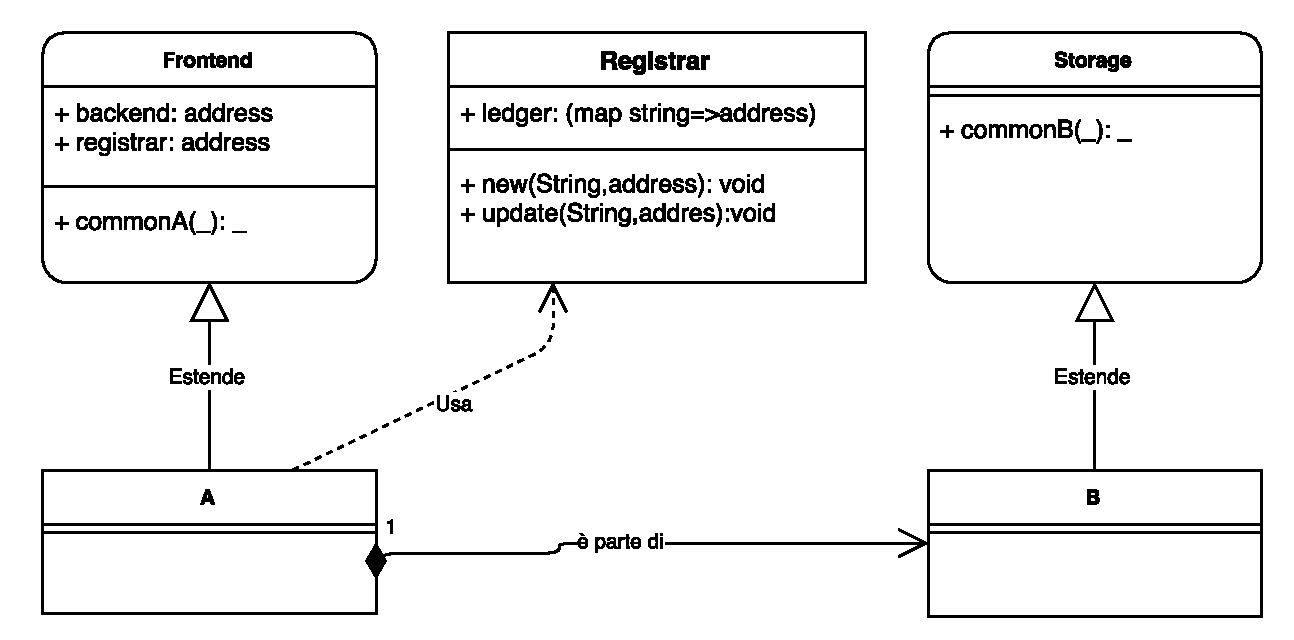
\includegraphics[width=0.75\textwidth]{System-of-contracts.pdf}
		\label{fig:system-of-contracts}
	\end{figure}

	Supponendo che il contratto Registrar è già operativo sulla blockchain, si scrive il codice per il contratto B, si esegue il deploy e l'indirizzo così ottenuto viene associato ad un nome simbolico nel contratto registrar. Viene caricato sulla blockchain il contratto A con l'indirizzo del contratto Registrar e il nome simbolico del contratto che implementa Storage.
	Nel contratto A ogni chiamata del metodo \lstinline|A.commonA()| scatena l'interrogazione del Registrar (\lstinline|registrar.ledger(backend)|) che come risultato da l'indirizzo sempre aggiornato del contratto Backend a cui deve invocare il metodo  \lstinline|commonB()|. In questo modo nel momento in cui il proprietario dell' applicazione vuole aggiornare solo la componente inclusa nel contratto B, caricherà un nuovo contratto sulla blockchain, salverà l'indirizzo di deploy nel registrar e da quel momento in poi A eseguirà il metodo del nuovo contratto.
	
	
	\subsubsection{Controlli temporizzati}\label(sssec:controllitemporizzati)
	
	Come affrontato nel sottocapitolo \ref{ssec:prolemibasatisublockchain} non esiste un meccanismo, decentralizzato ed interno alla blockchain, in Ethereum per implementare un sistema temporizzato o che reagisca ad eventi basati sullo stato dell'esecuzione dei contratti. Una frequente soluzione consiste nel fornire degli incentivi per spingere gli utenti a verificare loro stessi se si è verificato un determinato evento e impedendo che possano, allo stesso tempo, di "ingannare" il contratto per accaparrarsi l'incentivo.\\
	La funzione che, in Digichain, avrebbe bisogno di essere automatizzata è la rivalsa del contratto legata al contratto Registrazione che può trovarsi in uno stato in cui il costo $c$ accumulato nel tempo ha superato il bilancio $b$ del contratto Registrazione. La chiamata \lstinline|digichain.rivalsa(_intestatario)| è una funzione con side-effect il che comporta, anche in minima parte un costo. Questo scoraggia le persone a voler invocare la funzione, che scalerebbe degli Ether dai loro bilanci per sbloccare il pagamento verso qualcun'altro. Al contrario il controllo dell'ammontare della quantità di valuta che deve essere rimborsata viene eseguito tramite una call sullo stato del nodo locale, il che non comporta alcun costo in termini di transazioni (Si veda appendice \ref{appendice:b}). 
	
	Per aggiungere questa funzionalità e, quindi, creare degli incentivi verso gli utenti che riscuoterebbero i bilanci tramite \lstinline|.rivalsa(_intestatario)| si potrebbe aggiungere in fase di istanziazione dell'opera un nuovo valore $incentivo$ che il creatore dell'opera è disposto a pagare per il servizio di rivalsa fornito. 
	Da notare che attualmente la rivalsa è consentita solo al possessore dell'opera, ma per via della natura della funzione, incide in minima parte sul suo bilancio.
 
	


	
	
	

	\clearpage
	\section{Conclusioni}
%atrent letto il 30/3/17

Lo sviluppo dell'applicazione \text{Digichain} mi ha permesso di effettuare un primo approccio al linguaggio Solidity ed ai nuovi linguaggi orientati ai contratti. Studiando le possibili implementazioni già esistenti e i pattern riguardanti gli smart contract è stato chiaro che le tecnologie basate su blockchain ed in particolare Ethereum, sono realmente fruibili per applicazioni reali.

Se attualmente la rete di Ethereum ospita un carico moderatamente basso di transazioni al secondo\footnote{Attualmente durante l'impiego della pow dall' 1 alle 15 tx/s visionabile \url{https://etherchain.org/} e in accordo con \url{https://github.com/ethereum/wiki/wiki/Sharding-FAQ}}, con i recenti sviluppi del nuovo sistema di consenso \textit{Casper} e mediante lo sharding della blockchain, si stima di riuscire a moltiplicare di diverse centinaia il throughput attuale delle transazioni.  
Questo porterebbe la grande possibilità, nel prossimo futuro, alla sostituzione nelle applicazioni della terza parte fidata con uno smart contract autonomo, imparziale che non può essere soggetto a censura, frodi e periodi di downtime.  

L'applicazione è funzionante e può essere un punto di partenza per ulteriori sviluppi riguardanti l'interazione mediante interfacce web. Una possibile interazione con i browser, attraverso plug-in, potrebbe permetterebbe la verifica automatica del diritto d'uso delle opere digitali contenute in un sito.
 
Se da una parte lo sviluppo del progetto Ethereum sia ancora nel pieno sviluppo dall'altra, le enormi potenzialità che introduce e la facilità con cui uno sviluppatore può creare un'applicazione decentralizzata basata su blockchain rappresentano una realtà da approfondire.
	
Sono certo che, nel futuro, sempre più attenzione verrà data a questa tecnologia, non solo dal punto di vista del mero aspetto speculativo delle criptovalute o di particolari \textit{killer application}, ma le ricerche e gli sviluppi sulle proof, gli algoritmi di consenso e le nuove soluzioni getteranno le basi teoriche e pratiche dei nuovi sistemi decentralizzati.

	
	\clearpage
	\begin{appendices}
	Qui saranno contenute le appendici che nel corso della trattazione di questa tesi mi hanno permesso di eseguire operazioni particolari o che non hanno trovato posto nella trattazione.
	
	
	\section{Visionare i nodi di una private-net Ethereum mediante strumenti visuali}\label{appendice:a}
	%https://github.com/paritytech/parity
	
	Visionare lo stato di una blockchain non è un compito semplice da effettuare da riga di comando, si perde la visione d'insieme che spesso è la cosa che interessa. Potrebbe capitare di essere interessati all'hashrate della rete o al numero di transazioni che vengono effettuate in una particolare \textit{testnet}. Per visionare le blockchain pubbliche esistono siti costruiti ad hoc \footnote{I più celebri: \url{https://blockchain.info/}, \url{https://chain.so}, \url{.blockr.io},  \url{https://etherchain.org/}, \url{http://moneroblocks.info/}}per controllare graficamente lo stato dei blocchi, dei parametri riguardanti i blocchi e le transazioni, per ricevere notifiche real-time sulle transazioni immesse nella rete, però possiamo osservare che non per tutte le criptovalute questo è disponibile.\\
	Nel seguente caso vogliamo costruire un interfaccia grafica che permetta di osservare la blockchain privata di Ethereum.
	In rete, attualmente, è disponibile \textit{etherchain-light}\footnote{\url{https://github.com/gobitfly/etherchain-light}} che fornisce alcune delle funzionalità sopra citate e sfrutta l'interfaccia fornita da il light-node \textit{Parity}\footnote{\url{https://github.com/paritytech/parity}}.
	
	Nel seguente elaborato per costruire la rete privata di nodi sono state usate istanze Geth e per collegare il nodo Parity ad esse è stato richiesto di effettuare i settaggi del blocco di genesi, del network-id e l'aggiunta degli endpoint \lstinline|enode| dei nodi Geth. 
	Purtroppo per via dell'incompatibilità tra Parity e Geth è stato imposto il bisogno di tradurre il blocco di genesi per Geth in un formato compatibile per Parity\footnote{\url{https://github.com/keorn/parity-spec}}. Non è stato raggiunto il fine di far comunicare il nodo Parity con i nodi Geth e quindi non si è potuta analizzare la blockchain privata. Si sospetta fortemente che i nodi delle due tipologie non si sincronizzino per via del blocco di genesi diverso.\\
	
	Un applicativo parzialmente funzionante (durante la stesura di questo testo), ma che consente di visionare lo stato della rete a cui è connesso il nodo sottostante è \textit{ETHExplorer}\footnote{\url{https://github.com/carsenk/explorer}}. Esso non richiede il collegamento ad un nodo Parity, bensì si collega direttamente all'interfaccia RPC di Geth e quindi può essere utilizzato, senza aggiunte, nella topologia di rete di questo elaborato.
	
	Una volta scaricato l'applicativo e settato l'ambiente per consentirne la sua funzione, si eseguono le istanze dei nodi e l'applicativo si connette di default all'endpoint  \lstinline|localhost:8545|. 
	Navigando dal browser su  \lstinline|localhost:3000| è possibile avere delle statistiche sul tempo medio di creazione dei blocchi, l'hashrate attuale della rete e altri parametri, nonchè gli ultimi blocchi minati e le ultime transazioni effettuate.\\
	
	Attualmente questi strumenti non sono così completi rispetto ai siti di ispezione delle blockchain pubbliche (es. \url{blockchain.info}) ma forniscono un ottimo e immediato resoconto generale.
	
	\section{Inizializzazione di nodi Geth}\label{appendice:b}
		
		
		Per poter minare blocchi, includendo le transazioni e rispondendo alle chiamate via RPC, si necessita di una componente software che funga da nodo, le scelte sono molteplici. E' presente in rete \textit{Testrpc}\footnote{\url{https://github.com/ethereumjs/testrpc}}, un node scritto in puro javascript, il quale consente di predisporre delle interfacce e i comportamenti che permettono di simulare l'interazione con la blockchain ottenendo una rete privata composta da un solo miner. La grande quantità di funzioni dell'interfaccia che un nodo vero dovrebbe predisporre, rispetto a quella fornita da \textit{Testrpc}, porta questo software ad essere abbandonato durante lo sviluppo. 
		I programmi ufficiali che comunicano con la rete p2p, minano blocchi eseguendo la proof e predispongono un'interfaccia RPC completa possono essere trovati \url{https://github.com/ethereum/}. 
		In questo caso si è voluto utilizzare \textit{Geth}.
		Per simulare un applicazione su reti reali possiamo partecipare alla blockchain pubblica in rete semplicemente eseguendo:
		
		\begin{lstlisting}
		$ geth
		\end{lstlisting}
		
		in modo tale da scaricare tutti i blocchi e abilitare il mining sfruttando la modalità full-node. Esistono anche altre possibilità tra cui scaricare la blockchain solo per analizzarla o per connettersi ad un light-client che connettendosi ad altri nodi permette di interagire con la blockchain.
		
		Oltre a connetterci alla rete principale (main-net) c'è la possibilità che Geth possa collegarsi alla rete di testing di Ethereum (\textit{Ropsten}) creata appositamente per permettere ai contratti di essere in esecuzione in una rete vera e propria senza eventuali costi .
		L'ultima possibilità è quella di creare una propria blockchain in un'ambiente isolato: una private-net.
		
		Prima di poter far comunicare due nodi di Ethereum e farli minare sulla stessa blockchain bisogna comprendere con che criterio un nodo può sostituire la propria blockchain, sulla quale stava lavorando, con una che reputa migliore ottenuta da un nodo a cui è connesso.
		
		Un nodo in ascolto nella rete può trovare nuovi nodi a cui connettersi per lavorare insieme, con il fine di estendere la medesima blockchain, solo se si verificano due ipotesi:
		\begin{itemize}
			\item i nodi devono essere nella stessa rete virtuale (--$networkid$).
			\item i blocchi di $genesi$ dei due nodi devono essere identici perché un nodo abbandoni la propria blockchain e la sostituisca con un'altra.
		\end{itemize}
		
		Prima di tutto bisogna creare un account che sarà quello la cui chiave pubblica andrà inserita nell'etherbase/coinbase. Se in geth non viene passato nessun parametro $--etherbase$ viene preso il primo account trovato nel $keystore$\footnote{https://github.com/ethereum/go-ethereum/wiki/Managing-Your-Accounts}.	
		
		Per prima cosa installiamo Geth da repo\footnote{\url{https://github.com/ethereum/go-ethereum}}.
		
		I blocchi in Ethereum sono formattati\footnote{A seconda del software la formattazione dei blocchi varia, per esempio i blocchi compatibili con Parity non lo sono per Geth e viceversa.} in $JSON$ il che permette la lettura e scrittura in modo semplice. La creazione del blocco di genesi può essere eseguita in forma testuale, non avendo bilanci pre-allocati presenta la seguente struttura:
		
		\begin{lstlisting}
		//file CustomGensis.json
		{
		"nonce": "0x0000000000000042",
		"timestamp": "0x0",
		"parentHash": "0x0000000000000000000000000000000000000000000000000000000000000000",
		"extraData": "0x0",
		"gasLimit": "0x8000000",
		"difficulty": "0x400",
		"mixhash": "0x0000000000000000000000000000000000000000000000000000000000000000",
		"coinbase": "0x3333333333333333333333333333333333333333",
		"alloc": {
		}
		}
		\end{lstlisting}
		
		La scelta del valore assegnato ai parametri è per la maggior parte arbitraria, gli unici parametri che è significativo settare sono:
		
		\begin{description}
			\item[parentHash]: solo per il blocco di genesi è uno scalare assegnato a zero.
			\item[alloc]: è un vettore di record di $<pubkey,numWei>$ e ne definisce la pre-allocazione di valute ai rispettivi account.
			\item[difficulty]: definisce la difficoltà relativa al primo blocco, la difficoltà dei blocchi successivi verrà determinata dal timestamp e dalla difficoltà del blocco precedente.
			\item[coinbase]: o etherbase, è l'indirizzo a 160bit che definisce a quale indirizzo le fee e il reward del blocco debbano essere trasferiti. Per il blocco di genesi può essere arbitrario in quanto verrà determinato dinamicamente dagli address dei miner.
			\item[altro]: ogni altro campo è arbitrario e possono essere modificati a piacere contribuendo ad aggiungere entropia per evitare che involontariamente due nodi minino sulla stessa blockchain.
		\end{description}
		
		
		Per simulare due processi che eseguono il mining sulla stessa macchina locale, dobbiamo tenere in considerazione che ogni istanza: 
		\begin{itemize}
			\item deve poter creare le proprie strutture dati, --$datadir$ deve avere un path assoluto unico.
			\item deve essere in ascolto su porte differenti (--$port$ e --$rpcport$).
			\item l'endpoint deve essere unico o può essere disabilitato (--$ipcpath$ o --$ipcdisable$).
		\end{itemize}
		
		Per comodità andiamo a definire degli script per l'inizializzazione dei nodi ($init.sh$)e degli script per l'avvio dei processi Geth.
		\iffalse
		\begin{lstlisting}
		\\nodo1
		geth --identity Node1 --etherbase 2a54983e9b648684676c4f78638654177cd4be6a --networkid 1234  --maxpeers 4 --datadir="chain"  -verbosity 6 --ipcdisable --port 30301 --rpc --rpcapi "db,eth,net,web3,personal" --rpcport 8101 --rpccorsdomain "*"  console --nat "any"  --autodag --preload "jsScript/function.js" 2>> ./chain/00.log
		
		\\nodo2
		geth --identity Node1 --etherbase 438dfd4dfd26a42961d878a1e27eb9f40abb0d19 --networkid 1234  --maxpeers 4 --datadir="chain"  -verbosity 6 --ipcdisable --port 30302 --rpc --rpcapi "db,eth,net,web3,personal" --rpcport 8102 --rpccorsdomain "*"  console --nat "any"  --autodag --preload "jsScript/function.js" 2>> ./chain/00.log
		
		\end{lstlisting}
		\fi
		
		Una volta avviati i due processi disporremo di una console in ambiente JS con dei moduli precaricati che ci permettono di interagire con il nodo a cui siamo connessi e con la blockchain.
		I nodi di una rete privata dovranno essere registrati l'uno all'altro in modo tale da permettere che i peer scambino informazioni riguardanti le transazioni e i blocchi minati.
		
		%per testing e verifica che i nodi si vedono
		
		\iffalse
		1>admin.nodeInfo
		1>enode:\\....................[::]
		
		2>net.listening
		2>net.peerCount 
		2>admin.addPeer("enode:\\ .......... ")
		2>admin.peers
		\fi
		
		Da console possiamo creare nuovi account che risiederanno nel nostro keystore locale (se il keystore viene perso o la passphrase dimenticata non è possibile il recupero).
		
		\begin{lstlisting}
		> personal.newAccount()
		Passphrase: 
		Repeat passphrase: 
		"newaddress 0x..."
		\end{lstlisting}
		
		
		\textbf{Compilare da solc a EVMbytecode}\\
		
		I contratti vengono eseguiti sulla EVM di ethereum sottoforma di bytecode.
		
		Per verificare che geth conosca la locazione del compilatore per il linguaggio solidity:
		
		\begin{lstlisting}
		eth.getCompilers()
		\\oppure eth.compile.solidity("")
		\end{lstlisting}
		
		E' possibile installarlo mediante \textbf{apt-get}. Oltre ad esso esiste \textit{Solc-js} che permette di compilare file \lstinline|*.sol| e di produrre \lstinline|*.sol.js| direttamente importabili dalla console di Geth, questo consente di automatizzare eventuale testing.
		\iffalse
		
		\begin{lstlisting}
		sudo add-apt-repository ppa:ethereum/ethereum
		sudo apt-get update
		sudo apt-get install solc
		which solc
		\end{lstlisting}

		Per settare a runtime il compilatore:
		
		\begin{lstlisting}
		> admin.setSolc("/usr/bin/solc")
		
		"solc, the solidity compiler commandline interface\nVersion: 0.4.10+commit.f0d539ae.Linux.g++\n"
		\end{lstlisting}
		%oppure aggiungo da riga di comando il compilatore mediante l'opzione --solc /usr/bin/solc
		\fi
				
		Se correttamente installato da in output:
		\begin{lstlisting}
		> eth.getCompilers()
		["Solidity"]
		\end{lstlisting}
		
		E' possibile ora compilare uno o più contratti da console:
		
\begin{lstlisting}
> comp= eth.compile.solidity("contract A {}")
{
	<stdin>:A: {
	code: 			"0x60606040523415600b57fe5b5b60338060196000396000f3006060604052",
	info: {
		abiDefinition: [],
		compilerOptions: "--combined-json bin,abi,userdoc,devdoc --add-std --optimize",
		compilerVersion: "0.4.10",
		developerDoc: {
			methods: {}
		},
		language: "Solidity",
		languageVersion: "0.4.10",
		source: "contract A {}",
		userDoc: {
			methods: {}
			}
		}
	}
}
\end{lstlisting}
		
		Dall'output \footnote{Nel caso specifico di solc versione 0.4.10 la compilazione produce un errore sulle label json utilizzando output["<stdin>:NOMEDELCONTRATTO"] \url{http://ethereum.stackexchange.com/questions/11912/unable-to-define-greetercontract-in-the-greeter- tutorial-breaking-change-in-sol/11915\#11915}}si può vedere immediatamente come deve essere gestita una Dapp:
		
		\begin{itemize}
			\item \textbf{code}: è il codice in bytecode del contratto compilato, conterrà il codice di \textit{init} e il codice di \textit{body}.
			\item \textbf{info}: contiene i metadati compreso l'abi, il nome e altre informazioni che, unite all'indirizzo di deploy, permettono alla libreria Web3 di predisporre di oggetti per l'interazione con i contratti deploiati.
		\end{itemize}
		
		\subsection{Deploy ed interazione del contratto}
		
		Una volta che i nodi sono funzionanti ed è possibile compilare correttamente i contratti, può essere eseguito il deploy degli smart contract e interagirci.
		
		La libreria Web3 svolge il processo di collegare l'indirizzo del contratto che risiede (conosciuto solo dopo la compilazione e il deploy)  e l'interfaccia abi che predispone i metodi che possiamo interrogare.
		
		Una delle tante proprierty dell'oggetto \lstinline|eth| caricato nella console di Geth è \lstinline|eth.contract(abi)| che consente di ottenere un oggetto fittizio linkato ad abi. Su questo oggetto a seconda delle operazioni da effettuare vengono predisposti due proprietà dell'oggetto:
		\begin{description}
			\item[.new()]: consente di eseguire una transazione specificandone i campi ed inserendo nel campo \lstinline|data:| il codice del contratto. Se la transazione avverrà, la callback sarà chiamata e l'istanza collegata al contratto sulla blockchain sarà restituita.
			\item[.at()]: consente di specificare un indirizzo e di ritornare un istanza del contratto che risiede sulla catena. 
		\end{description}
		
		In tutti e due i casi, ottenuta l'istanza sarà possibile invocare su di essa il nome della funzione (contenuta nell'abi) e specificare se si vuole eseguire una call o una transazione\ref{appendice:c}.

		
		\subsection{Mining}
		
		La forma più semplice di mining da effettuare con Geth è il mining via CPU e senza dover settare l'ambiente. Nella versione \textit{Frontier} l'intervallo tra un blocco e l'altro è bilanciato sui 15-17 secondi, bilanciato dalla difficoltà settata dalla PoW Ethash.
		
		\begin{lstlisting}	
		> miner.start(1)
		true
		
		>eth.hashrate
		4
		\end{lstlisting}
		
		Come argomento del comando \lstinline|.start()| viene specificato il numero di thread che il processo usa per il mining. Nel caso un nuovo peer si unisce al mining, della medesima blockchain della stessa rete, automaticamente la difficoltà viene alzata.
		
		\iffalse
		\begin{lstlisting}
		eth.getBlock("pending", true).transactions
		\end{lstlisting}
		\fi
	\section{SendTransaction (side-effect call) e call}\label{appendice:c}
	
	Formalmente i metodi \lstinline|.sendTransaction()| e \lstinline|.call()| che possiamo eseguire su un istanza \lstinline|eth.contract| mandando entrambi due chiamate all'interfaccia rpc del nodo a cui siamo collegati tramite l'interfaccia \textit{web3} (e i relativi moduli) che è caricata nella console JS. Il primo metodo esegue una transazione: viene passata all'interfaccia il mittente della transazione firmandola, il payload data, il nonce e tutti gli altri parametri di una transazione. L'esecuzione del comando ritornerà sempre l'hash della tx. Viceversa il metodo \lstinline|.call()| può essere invocato su un metodo che non produce cambiament e viene eseguita dal nodo sottostante, ritornerà un valore se sarà specificato le clausole \lstinline|constant returns|\footnote{L'identificativo \lstinline|constant| dichiara che la funzione non ha side-effect, questo rafforza l'analisi formale che può essere fatta}. 
	Questo comporta:
	\begin{itemize}
		\item la transazione prima di produrre un cambiamento di stato deve essere condivisa con gli altri nodi e inclusa in un blocco valido, non è possibile a priori, sapere ne quando ne se sarà inclusa. 
		\item la call ispeziona solo lo stato dei contratti nella blockchain e può essere eseguita immediatamente, non produce effetti, non deve essere inclusa in un blocco e ciò comporta che la sua esecuzione non ha un costo in gas.
	\end{itemize}
	
	Ogni transazione nella piattaforma Ethereum ha un costo minino di 21000 gas (che moltiplicato per il gasPrice fornisce il costo in Wei della transazione)\footnote{ Per la documentazione ufficiale: \url{https://github.com/ethereum/wiki/wiki/JavaScript-API\#web3ethcall}}.
	
	\section{Eventi, log e return}\label{appendice:d}

	Ogni contratto ha associato una struttura dati che contiene le \textit{entry log} emesse da un contratto. In base a \cite{yellowpaperethereum} un log è formato dall' indirizzo del logger, una serie di campi di 32 byte e un campo data contenente un numero arbitrario di byte.
	
	Come risultato di un invocazione di un evento \lstinline|event NomeEvento(_type _param)| viene emesso e registrato un log. Ovviamente ogni singolo log e ogni byte in esso contenuto costano gas, ma se la notifica è indispensabile si ritiene obbligato la scrittura dei log\footnote{I log costano 375 gas ognuno e 8 gas ogni byte aggiunto contro i 20.000 gas per ogni byte di storage del contratto}.
	
	L'esecuzione di una transazione dalla console di Geth,visto che restituisce solo l'hash della tx inviata per le ragione dell'appendice \ref{appendice:b}, richiede per la restituzione di un valore dalla sua esecuzione l'utilizzo di eventi.
	
	La classe web3.eth.contract permette di porsi in ascolto sul log di uno specifico contratto, specificando uno o tutti gli eventi che predispone l'interfaccia abi\footnote{	\url{https://github.com/ethereum/wiki/wiki/JavaScript-API\#contract-events}}.
	
	\iffalse
	using a callback is just calling the RPC method asynchronously and will return the same as the sync function. On the RPC side there is no way to get a notification whether the tx was mined or not. you would need to check that yourself with a script looking at the next block.
	We could think of integrating this into web3.js, but thats out of scope for now.
	\fi

\end{appendices}
	\clearpage


	%% Bibliography .bib
	\bibliography{./Struttura/bib.bib}
	\bibliographystyle{unsrt}	
\end{document}
